\chapter[Active noise cancelling design]{Active Noise Cancelling System} \label{c:tc1} 

\section{Overview}

\begin{figure}[h]
\centering
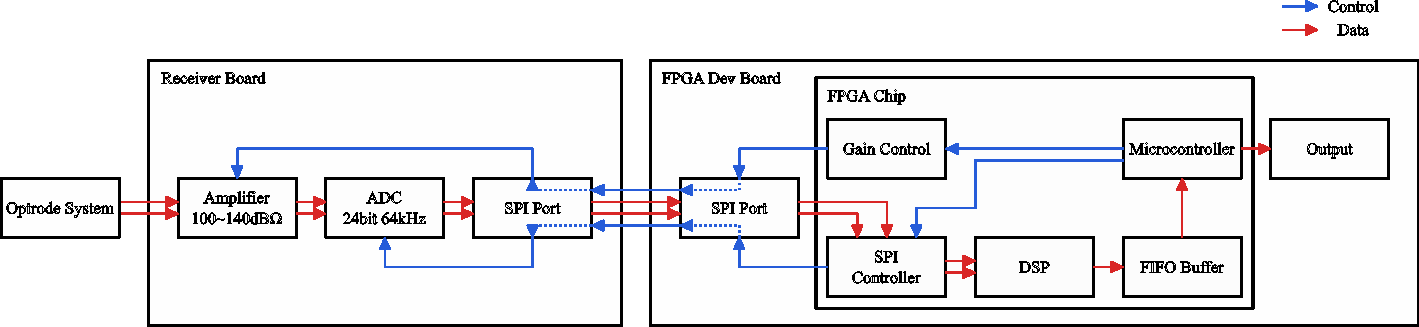
\includegraphics[width=0.9\linewidth]{4-ANC_Sys/ANCBlockDiagram.pdf}
\caption{ANC System Block Diagram}
\label{fig_ANCBlockDiagram}
\end{figure}

In the existing electro-optical detection system, a light source sends light towards an optrode transducer, where the light is modified to convey information sensed by nerve cell electrodes. The light is then delivered to a photodetector, which recovers nerve data from the modulated light.  From experiment data, the majority of the noise in the output signal comes from the light source.  Therefore, by placing a light splitter at the output of the light source, two light output channels with almost identical noise can be achieved.  Then the two light channels are connected to an active optrode and an inactive optrode, and the two channels from the photodiode receiver.  With this setup, one message channel would contain nerve signal and system noise, while the other noise channel only contains system noise.  By passing the two channel signals to an active noise cancelling algorithm, the noise in the message channel can be largely removed based on the information in the noise channel.

The current receiver board consists of photodiodes, variable gain DC coupled amplifiers, and variable gain AC coupled amplifiers.  This board converts light into an analogue voltage signal, then a data acquisition equipment converts the analogue signal to digital.  In this process, both the receiver board and the data acquisition equipment add noises to the signal.  To better remove the noise, higher noise correlation between the two channels is desired.  Since the base noise floor for the data acquisition equipment is fixed, increasing the gain in the receiver board would result in higher noise correlation.  The maximum gain this board can set without distorting the signal is 120dB.  More gain would result in an unstable output.  The nerve signal of interest is only in the AC part of the modulated light, which means the receiver board gain is limited by the DC coupled first stage amplifier.  

In this project, a PCB board that converts two channel light input to a noise reduced digital data output will be made.  This board contains a photodiode, amplifier, filter, analogue to digital converter, and an FPGA.  From the input side, the photodiode will be AC coupled before the first amplifier stage to achieve better gain and noise performance.  A maximum gain of 40dB for each amplifier stage is reasonable since a gain higher than that could distort the signal and possibly cause the amplifier to be unstable.  Therefore, to achieve a total gain of over 120dB, multiple stages are needed.  As the gain must be variable, digital potentiometers will be needed in the amplifier circuit to digitally control the gain in each stage.  A filtering circuit will be placed between the amplifier stages and the analogue to digital converter to avoid aliasing.  Then One or more analogue to digital converters will convert the filtered analogue signal to a digital signal and pass it to the FPGA via a serial port, for example SPI or I2C.  The nerve signal has a frequency band of interest from 10Hz to 10kHz, so the sampling frequency of the analogue to digital converter must be greater than 20kHz to satisfy the Nyquist rate.  Also, for higher accuracy, the analogue to digital converter should have more than 24 bits.

An algorithm is designed inside the FPGA to process the signal coming from the analogue to digital converter.  This algorithm is a mix of a simplified wiener filter and an adaptive filter, with around 5 to 10 filter coefficient taps.  Since the multiply and divide operations in the FPGA cost a lot of hardware resources, and the FPGA can run at over 100MHz, which is a lot faster than the signal sampling frequency, a pipeline structure can be made to reduce the size of the filter design.  The two inputs of this algorithm are a noisy nerve activity signal and a pure noise signal.  The noise in these two signals is largely correlated.  Assume the noisy nerve activity signal consists of nerve activity message m, correlated noise n, and uncorrelated noise n1, while the pure noise signal is consisting of correlated noise n, and uncorrelated noise n2.  The algorithm is designed to remove correlated noise n from the noisy nerve activity signal by using the noise information from the pure noise signal.  The simplified wiener filter compares the autocorrelation and crosscorrelation of these two signals and calculates a set of coefficients which filters the pure noise signal so that the uncorrelated noise n2 is removed.  The filtered pure noise signal is basically correlated noise n, by subtracting it from the noisy nerve activity signal, the noise reduction process is completed.

Fig.~\ref{fig_ANCBlockDiagram} shows the block diagram of the active noise cancelling system;  it consists of two boards: a receiver board and an FPGA development board.  The two signals are received by the receiver board, amplified with a maximum gain of~\qty{140}{dB\Omega}, and converted into digital signals.  The two digital signals are then processed using a noise-cancelling algorithm implemented on the FPGA development board which ultimately outputs a cleaner signal.


\section{Preliminary work}

\begin{figure}
\centering
\begin{subfigure}{.5\textwidth}
  \centering
  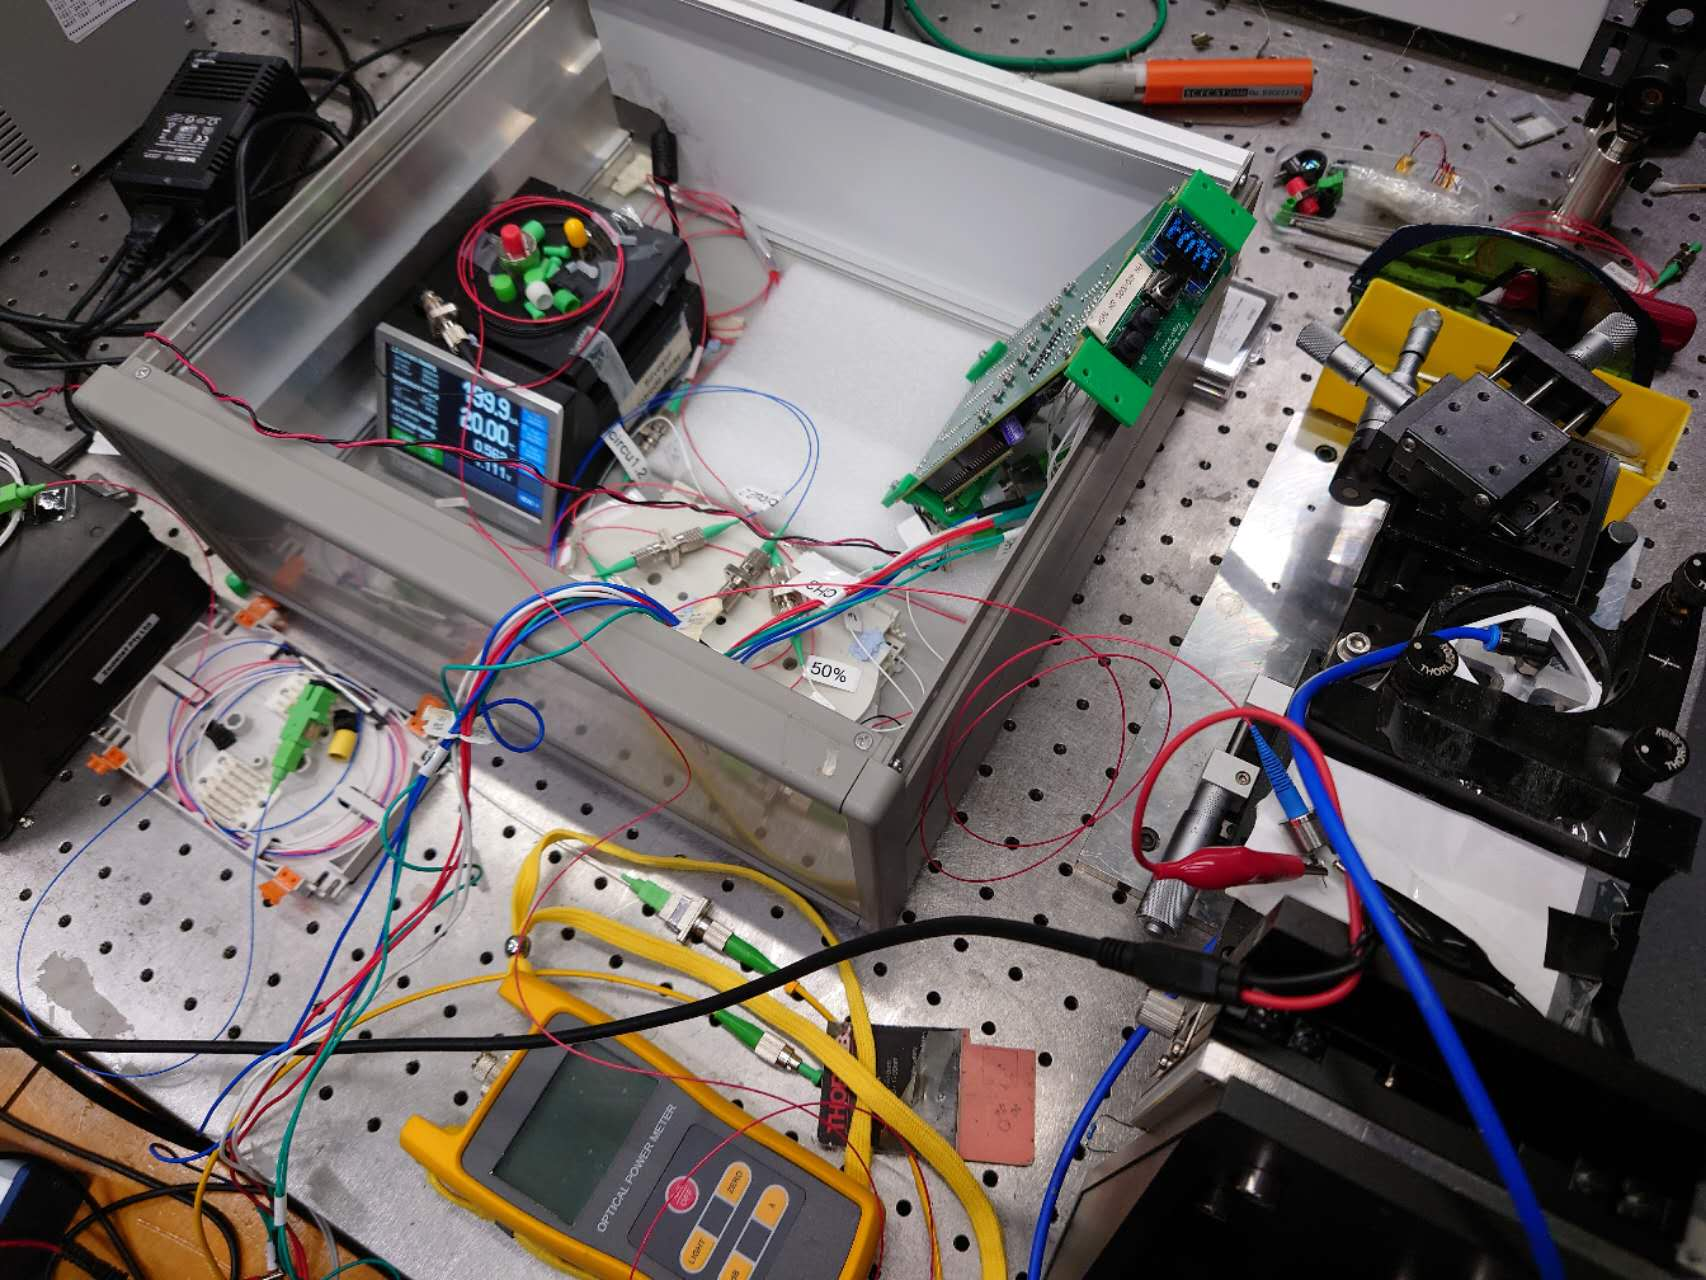
\includegraphics[width=0.9\linewidth]{4-ANC_Sys/OptrodeSys.jpg}
  \caption{}
  \label{fig_OptrodeSysPartial}
\end{subfigure}%
\begin{subfigure}{.5\textwidth}
  \centering
  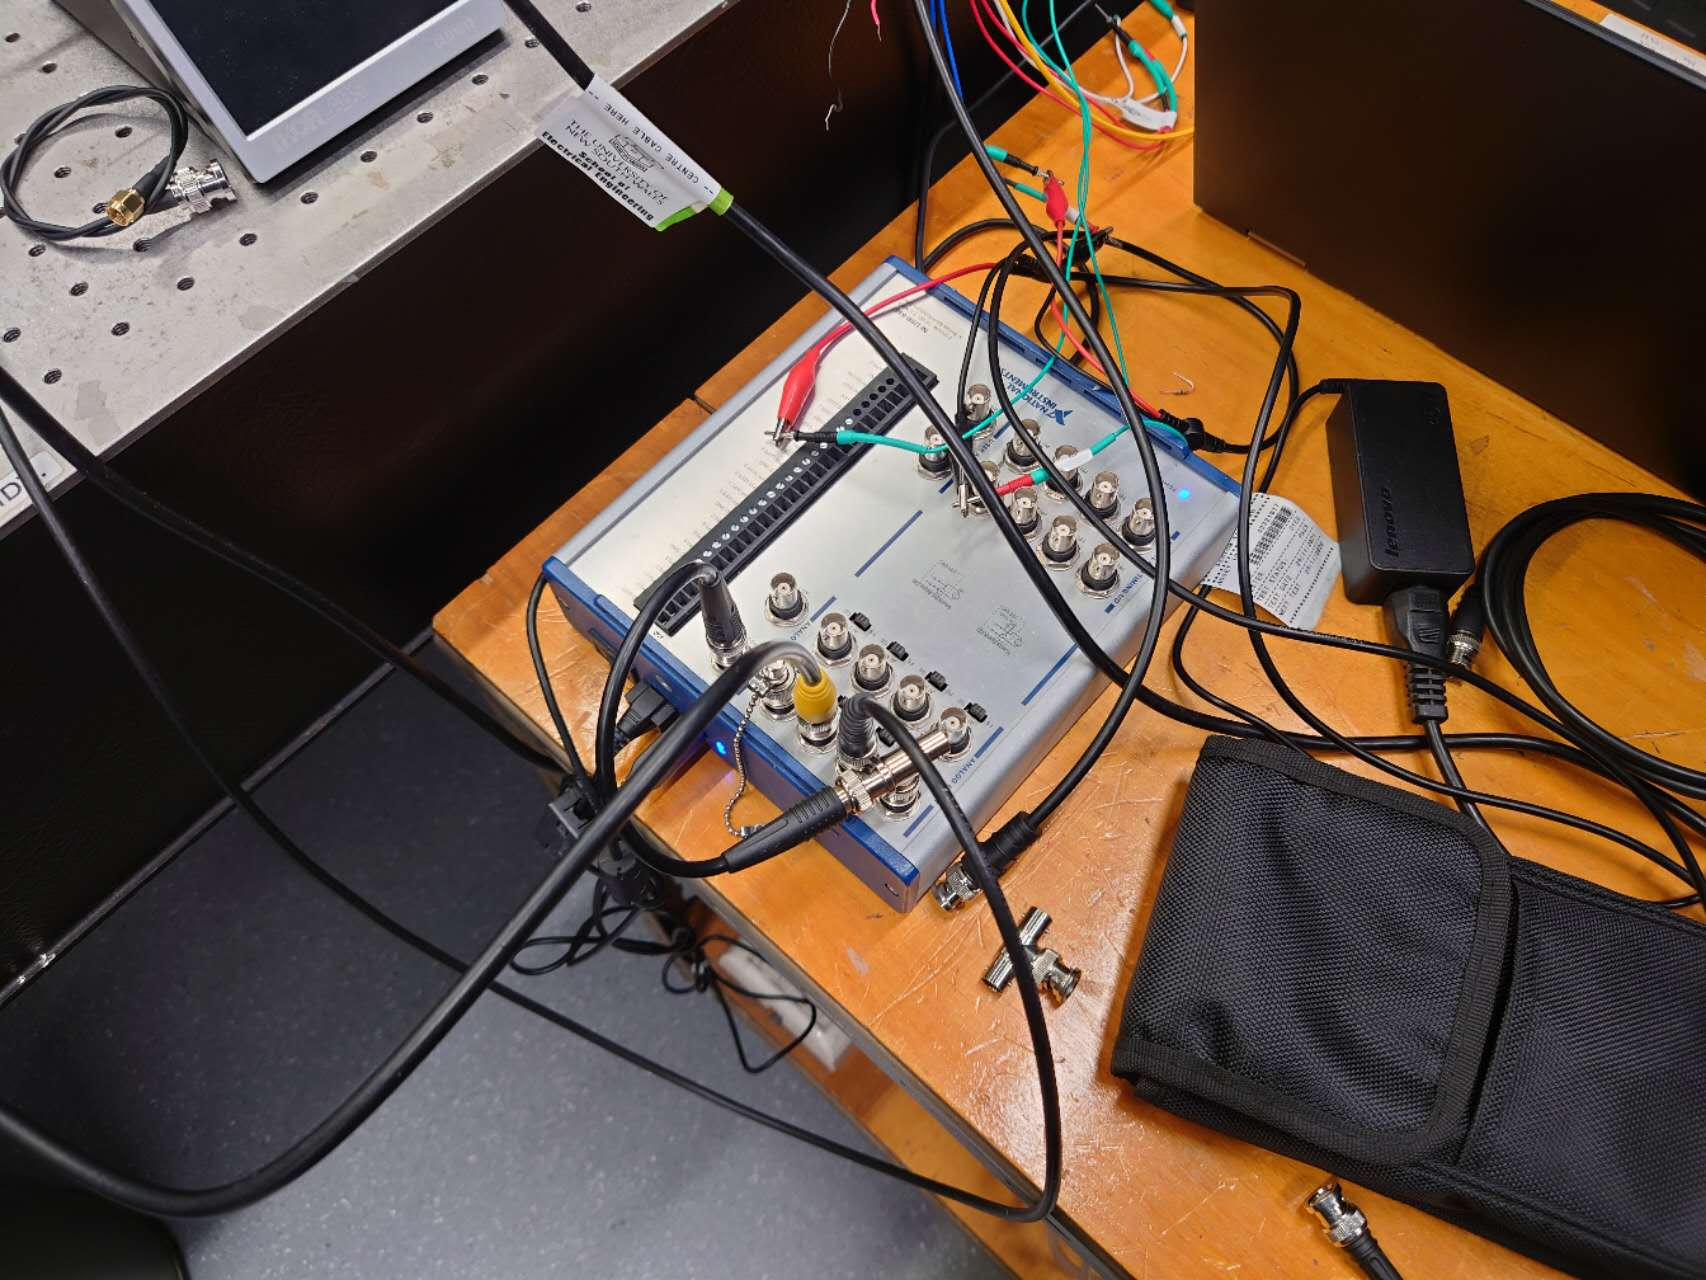
\includegraphics[width=0.9\linewidth]{4-ANC_Sys/DAQ.jpg}
  \caption{}
  \label{fig_DAQ}
\end{subfigure}
\caption{Optrode system (a) Light source, receiver board, and optrode (b) Data acquisition equipment}
\label{fig_OptrodeSys}
\end{figure}

Fig.~\ref{fig_OptrodeSys} shows the optrode detection system setup.  Fig.~\ref{fig_OptrodeSysPartial} shows the light source (black box on the top left), a light receiver board that was made previously (green PCB board), a light circuit (next to the light source and receiver board), and the optrode (grabbed by a red and a black alligator cable at the bottom right).  Fig.~\ref{fig_DAQ} shows the data acquisition equipment.

To confirm the possibility of using active noise cancelling on the optrode system, some measurement is undertaken to analyze.  In order for the active noise cancelling to work, most of the noise in the system must be generated before the active and inactive optrode, which means mostly from the light source.  Fig.~\ref{fig_CrossCoTest} shows four different setups for testing the noise added at each part of the system.  The first test fig.~\ref{fig_CrossCoTest} (a) put through the light into one channel on the receiver board, and one channel of output is then connected to two channels at the data acquisition equipment, the difference in the two-channel data is only caused by the difference of the two-channel of data acquisition equipment.  The second test fig.~\ref{fig_CrossCoTest} (b) put through the light to a light splitter and split into two identical lights, then to two channels at the light receiver board and two channels at data acquisition equipment.  The difference in output data here is the noise in both the receiver board and the data acquisition equipment.  The third test fig.~\ref{fig_CrossCoTest} (c) adds up two inactive optrodes between the light splitter and the light receiver board, and the fourth test fig.~\ref{fig_CrossCoTest} (d) adds inactive optrode to one channel and active optrode to another channel.  In these two tests, the difference in output data comes from optrodes, light receiver board, and data acquisition equipment.  For these tests, there is no signal input at any optrodes.  The two-channel digital output at each test should contain the same noise from the light source, and different noise from other parts of the circuit.  To compare the results, the cross-correlation of the four tests is plotted.

\begin{figure}[h]
\centering
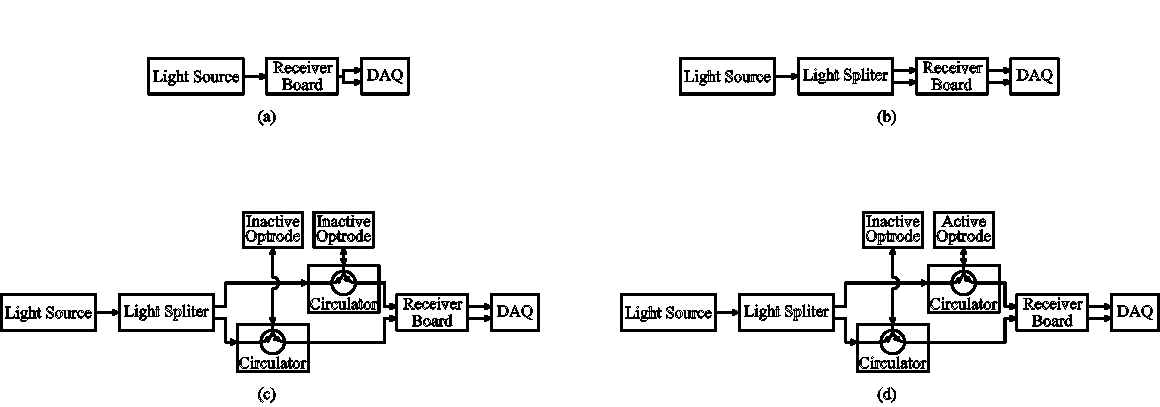
\includegraphics[width=0.9\linewidth]{4-ANC_Sys/CrossCoTest.pdf}
\caption{Cross correlation test (a) Test 30, inactive split to DAQ, receiver board (b) Test 32, inactive 2 split to receiver, receiver board (c) Test 35, inactive 1 and 2, receiver board (d) Test 36, active and inactive, receiver board}
\label{fig_CrossCoTest}
\end{figure}

Fig.~\ref{fig_CrossCorrelationTest} shows the results of cross-correlation for the two output data on each of the four test setups in fig.~\ref{fig_CrossCoTest}.  Fig.~\ref{fig_CrossCorrelation30} shows a normalised cross-correlation of \qty{0.719}{}, fig.~\ref{fig_CrossCorrelation32} shows \qty{0.711}, fig.~\ref{fig_CrossCorrelation35} shows \qty{0.538}, and fig.~\ref{fig_CrossCorrelation36} shows \qty{0.622}.  The normalised cross-correlation is an algorithm for two signals, the result ranges from \qty{-1}{} to \qty{1}{}, that \qty{1}{} means two identical signals, \qty{-1}{} means two reversed signals, and \qty{0}{} means two uncorrelated signals.  Our results show that the light receiver board generates a very small amount of noise, the data acquisition equipment and the optrodes generate some noise, but compared to the noise from the light source, they are still relatively small.  This indicates the possibility of using active noise cancelling method to reduce noise in the optrode system.

\begin{figure}[H]
\centering
\begin{subfigure}{.5\textwidth}
  \centering
  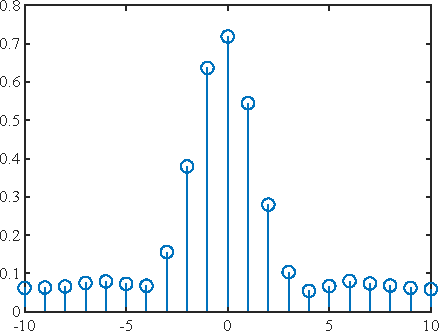
\includegraphics[width=0.8\linewidth]{4-ANC_Sys/CrossCorrelation 30.pdf}
  \caption{}
  \label{fig_CrossCorrelation30}
\end{subfigure}%
\begin{subfigure}{.5\textwidth}
  \centering
  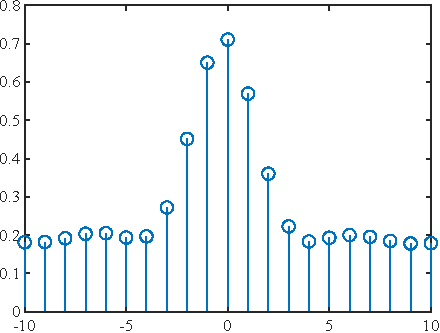
\includegraphics[width=0.8\linewidth]{4-ANC_Sys/CrossCorrelation 32.pdf}
  \caption{}
  \label{fig_CrossCorrelation32}
\end{subfigure}
\begin{subfigure}{.5\textwidth}
  \centering
  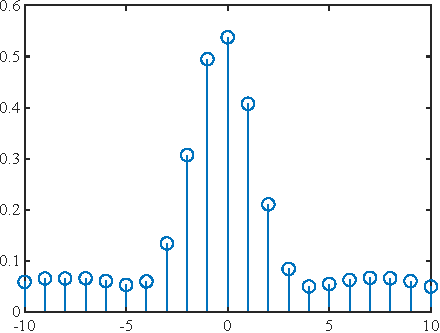
\includegraphics[width=0.8\linewidth]{4-ANC_Sys/CrossCorrelation 35.pdf}
  \caption{}
  \label{fig_CrossCorrelation35}
\end{subfigure}%
\begin{subfigure}{.5\textwidth}
  \centering
  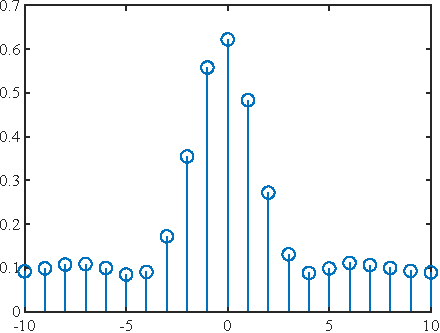
\includegraphics[width=0.8\linewidth]{4-ANC_Sys/CrossCorrelation 36.pdf}
  \caption{}
  \label{fig_CrossCorrelation36}
\end{subfigure}
\caption{Cross correlation test on different parts of optrode system (a) Test 30, inactive split to DAQ, receiver board (b) Test 32, inactive 2 split to receiver, receiver board (c) Test 35, inactive 1 and 2, receiver board (d) Test 36, active and inactive, receiver board}
\label{fig_CrossCorrelationTest}
\end{figure}



\section{Reveiver Board}

\subsection{Previous board}

\begin{figure}[h]
\centering
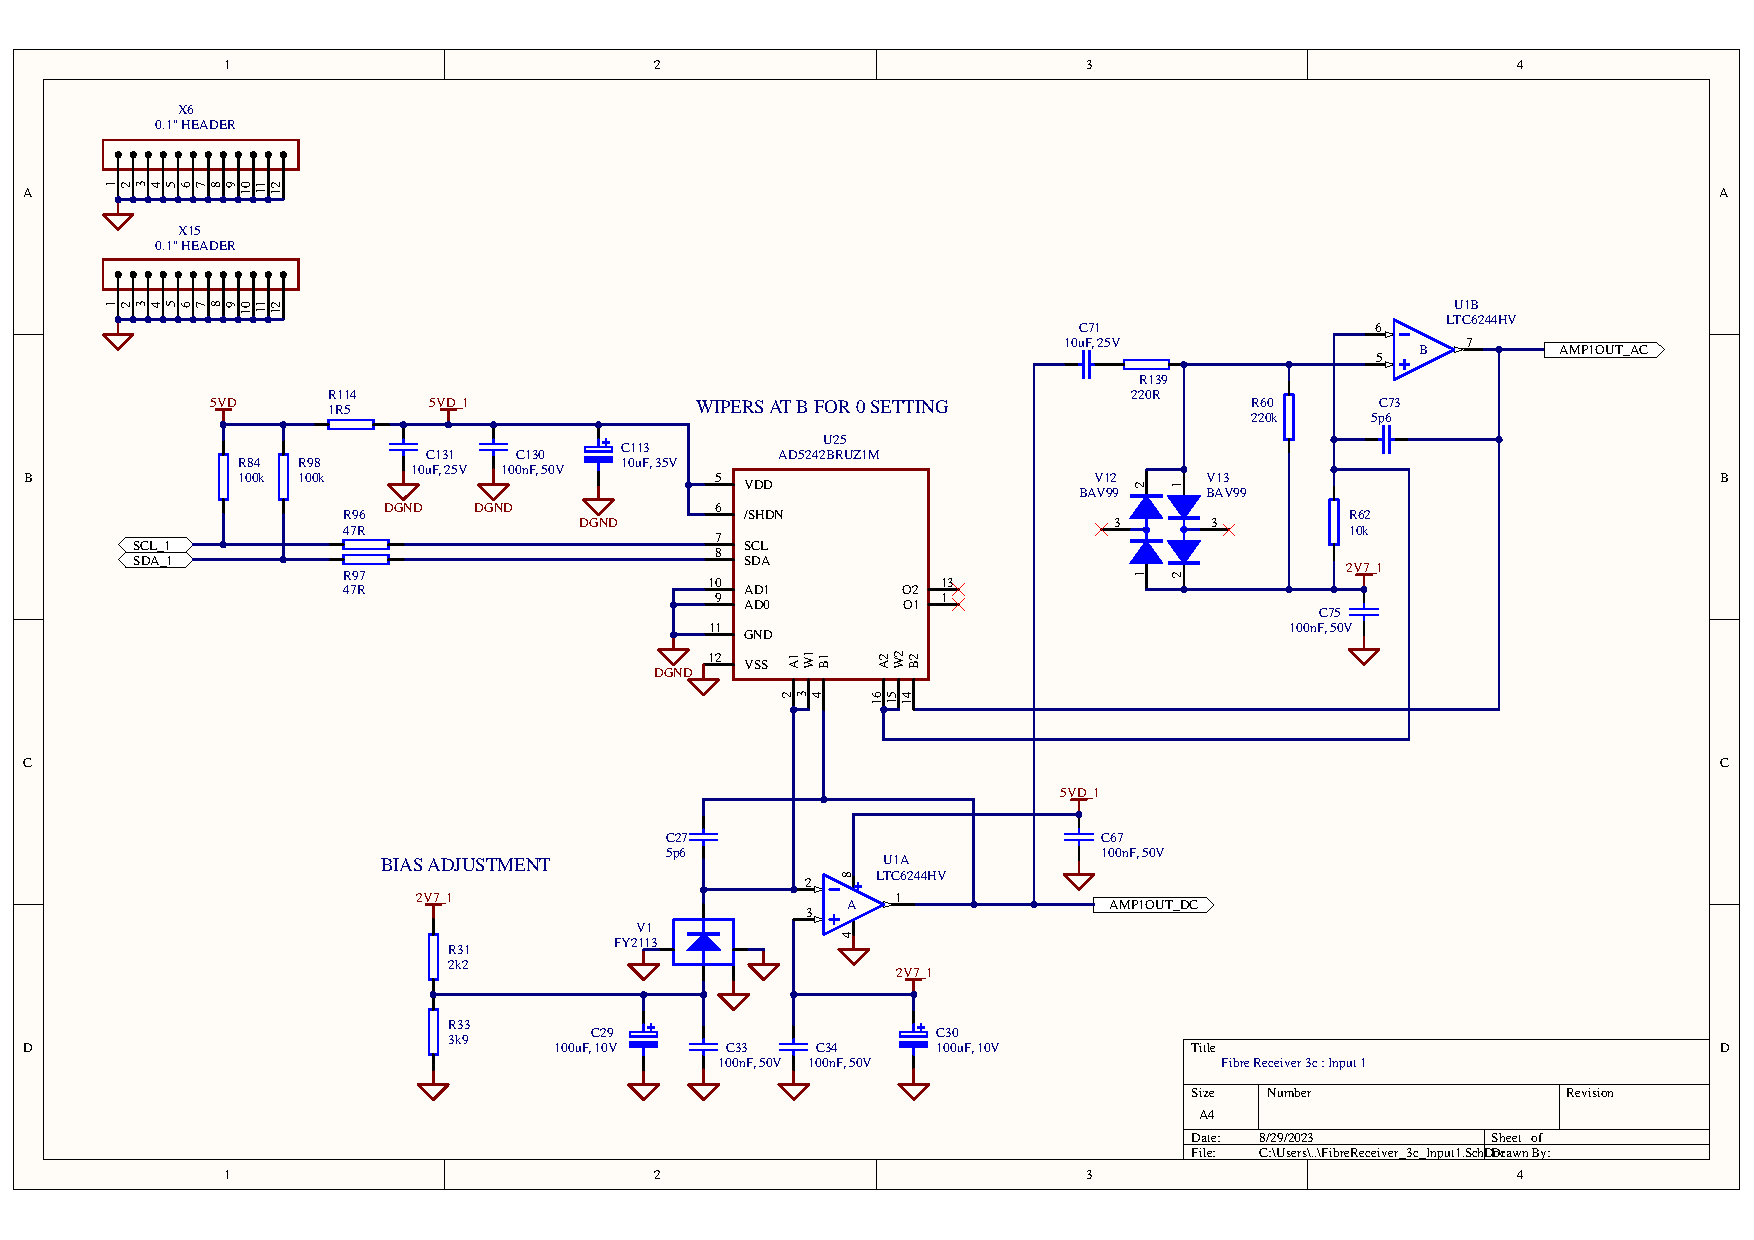
\includegraphics[width=0.9\linewidth]{4-ANC_Sys/FibreReceiver_3c_Input1.pdf}
\caption{Previous board (1)}
\label{fig_DavidBoardIn}
\end{figure}

\begin{figure}[h]
\centering
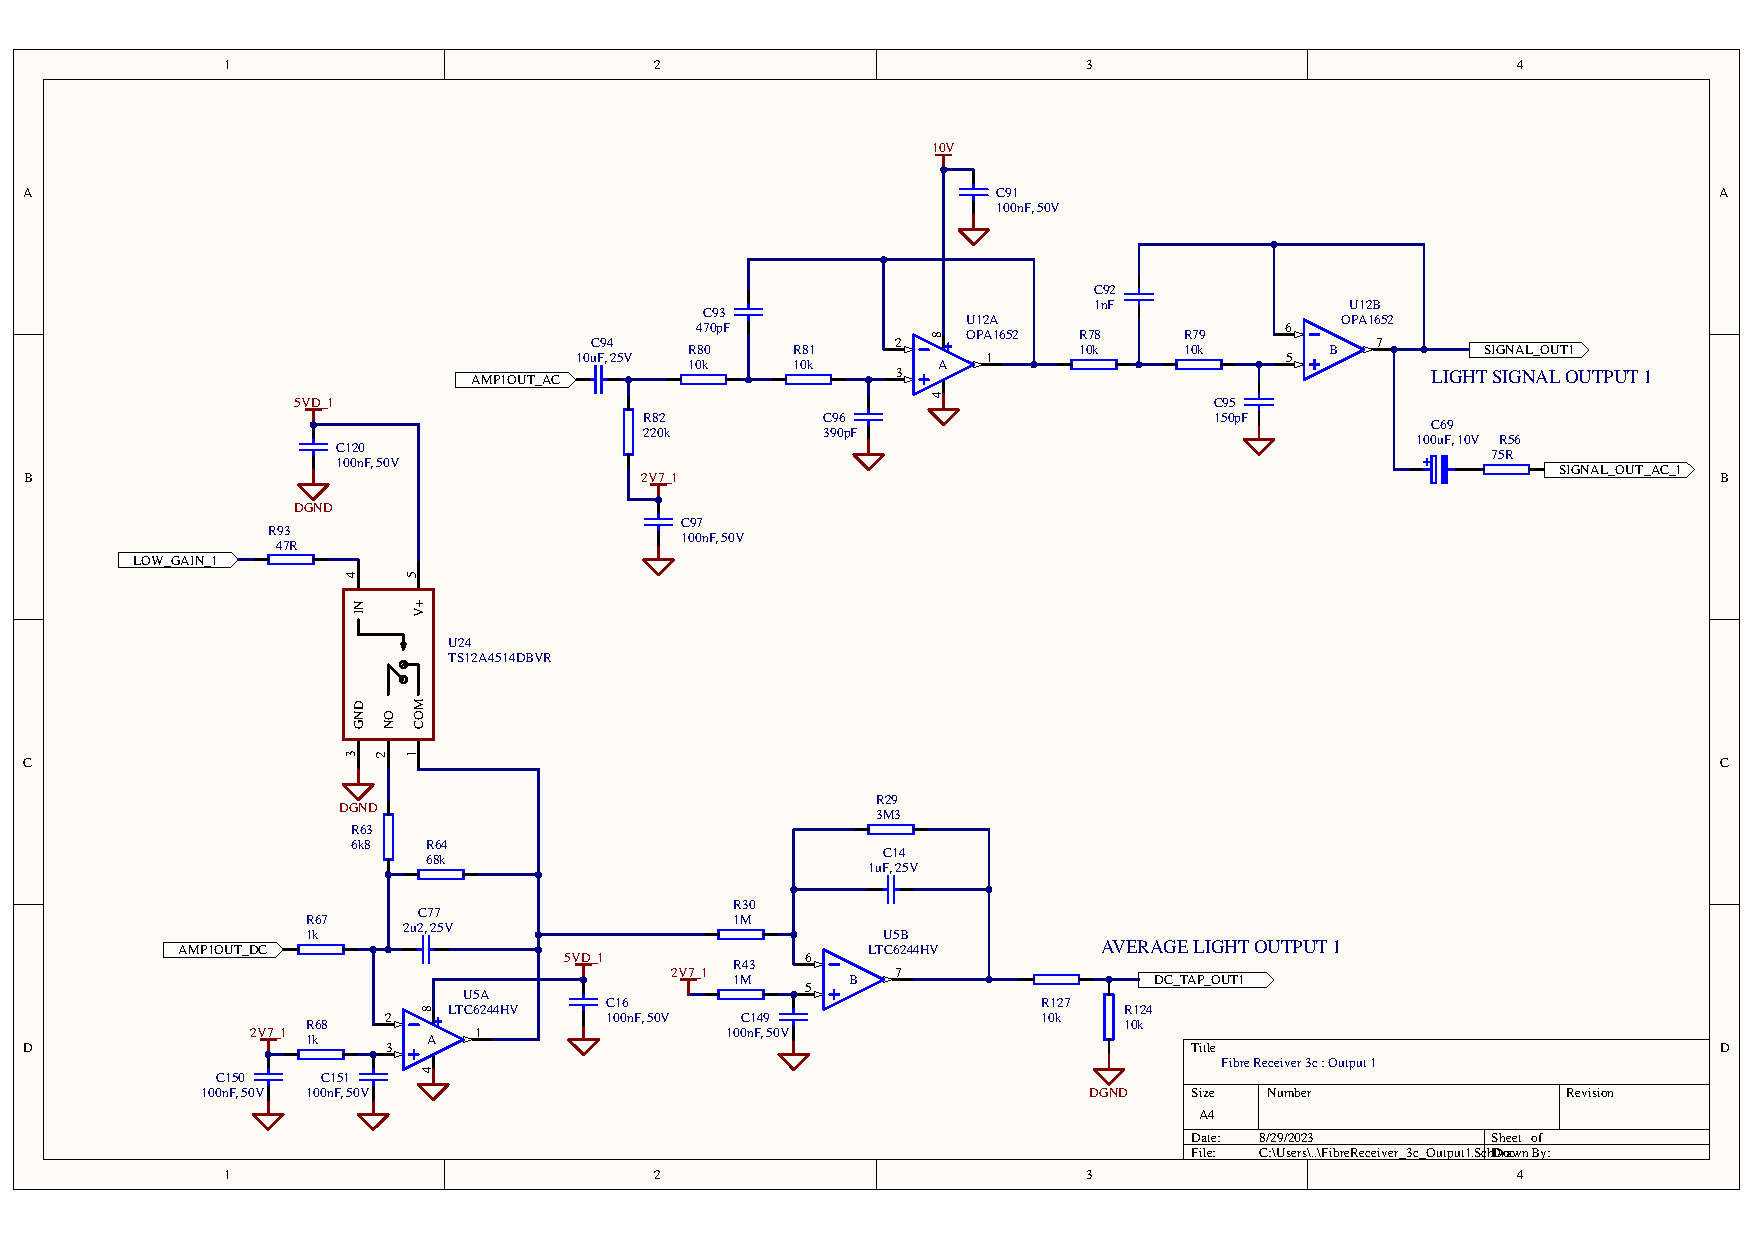
\includegraphics[width=0.9\linewidth]{4-ANC_Sys/FibreReceiver_3c_Output1.pdf}
\caption{Previous board (2)}
\label{fig_DavidBoardOut}
\end{figure}

In previous optrode experiments, a light receiver board was used to convert light into voltage signal.  This previous receiver board has four light channels input, fig.~\ref{fig_DavidBoardIn} and fig.~\ref{fig_DavidBoardOut} show one of the four channel circuit schematic.  In fig.~\ref{fig_DavidBoardIn}, a reverse biased photodiode is connected to a transimpedence amplifier, which amplifies the current coming out of the photodiode to voltage.  Then a capacitor AC couples the output of the transimpedence amplifier, and a non-inverting amplifier (biased at \qty{2.7}{V}) amplifies the AC part of the signal further.  The gain of both the transimpedence amplifier and the non-inverting amplifier is variable by a digital potentiometer.  The bottom half of fig.~\ref{fig_DavidBoardOut} shows further processing to the DC part of the signal, which is the output of transimpedence amplifier, and that part is not of our interest.  The upper half of fig.~\ref{fig_DavidBoardOut} shows a fourth-order low-pass filter, which is designed for anti-aliasing.  On this board, light comes in from fibre and converts to current at the photodiode, and then amplified to voltage at the transimpedence amplifier and non-inverting amplifier, then is passed to the anti-aliasing filter, and finally arrives the output of the board.  A data acquisition equipment is connected to the output of the board to record the output voltage signal and convert it into a digital signal to a computer.

This board is capable of amplifying the signal up to \qty{120}{dB} gain.  However, when set the gain to \qty{140}{dB}, the output of the transimpedence amplifier is saturated.  In the light that comes into the photodiode, the majority part is DC, and only a very small portion of the light contains AC signal that is modulated at the optrode.  Therefore, a higher gain can be achieved by AC couple the photodiode before transimpedence amplifier.

The previous light receiver board was made for another project that is not relevant to optrode, therefore some specifications are not optimised for optrode measurement.  In this project, a new light receiver board is designed and made, which has higher gain, lower noise, and digital output ability compare to the previous light receiver board.

\subsection{New light receiver board}

\begin{figure}[h]
\centering
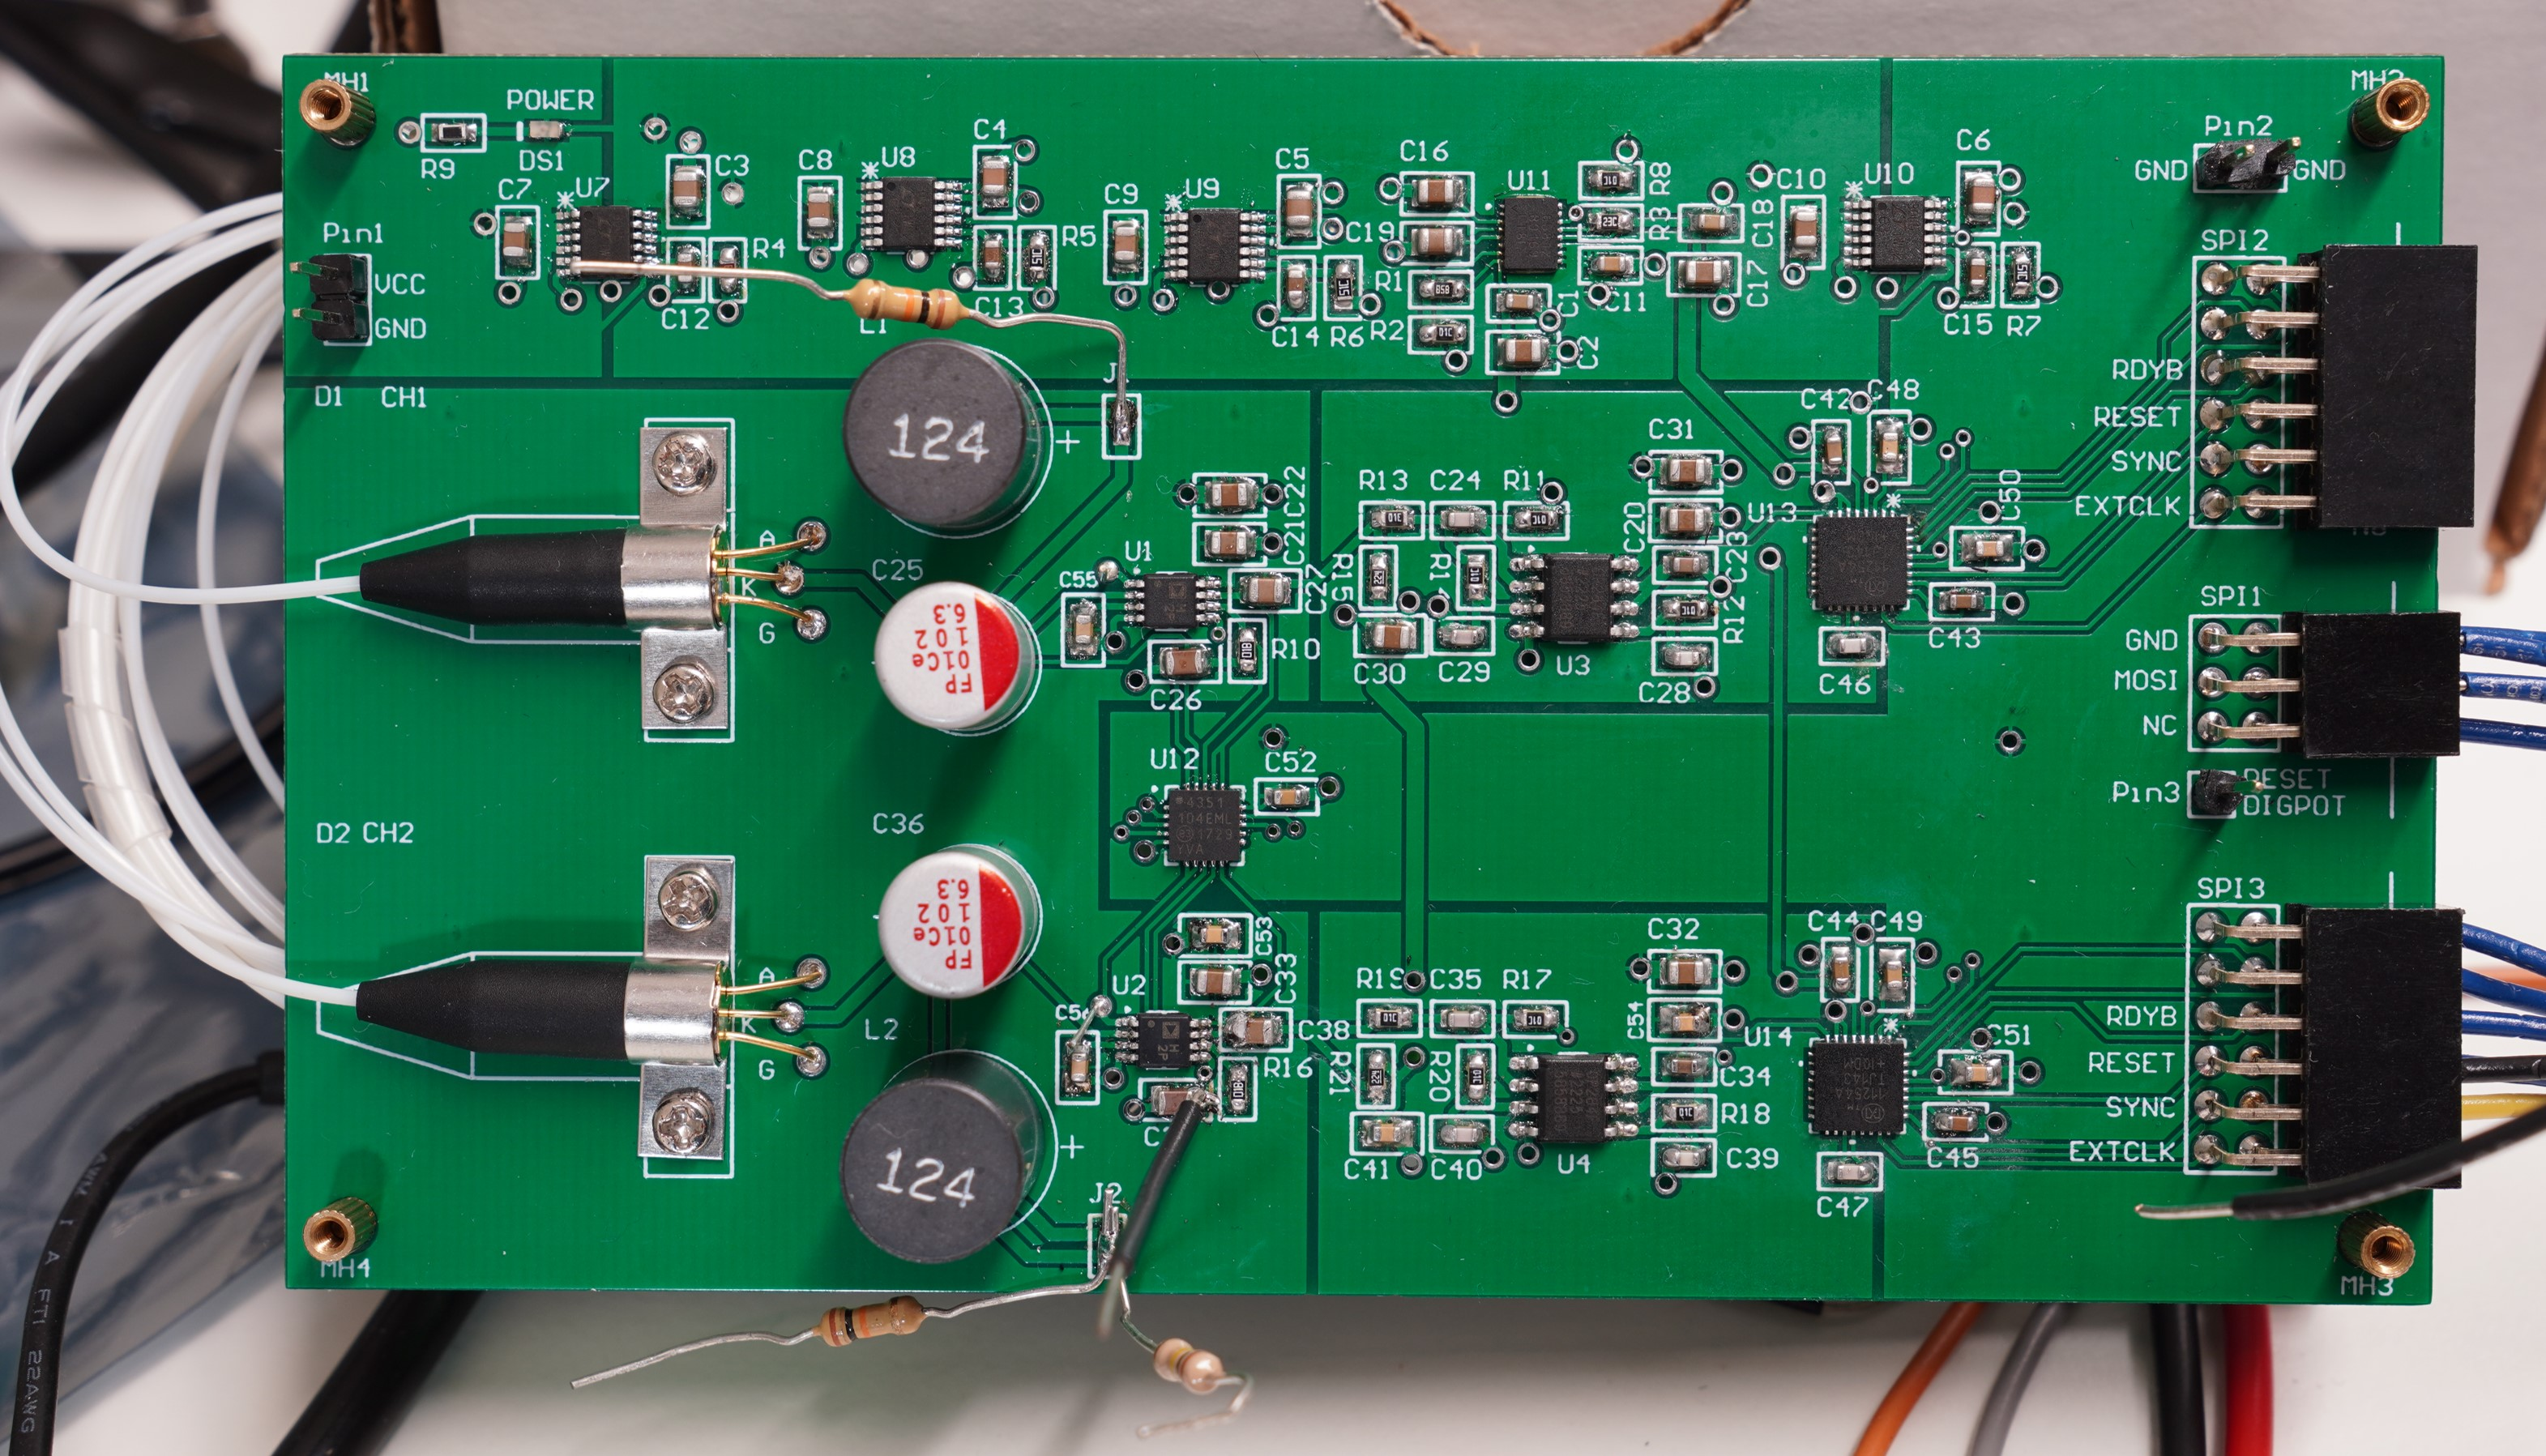
\includegraphics[width=0.9\linewidth]{4-ANC_Sys/ReceiverBoard.jpg}
\caption{Receiver Board}
\label{fig_ReceiverBoard}
\end{figure}

\begin{figure}[h]
\centering
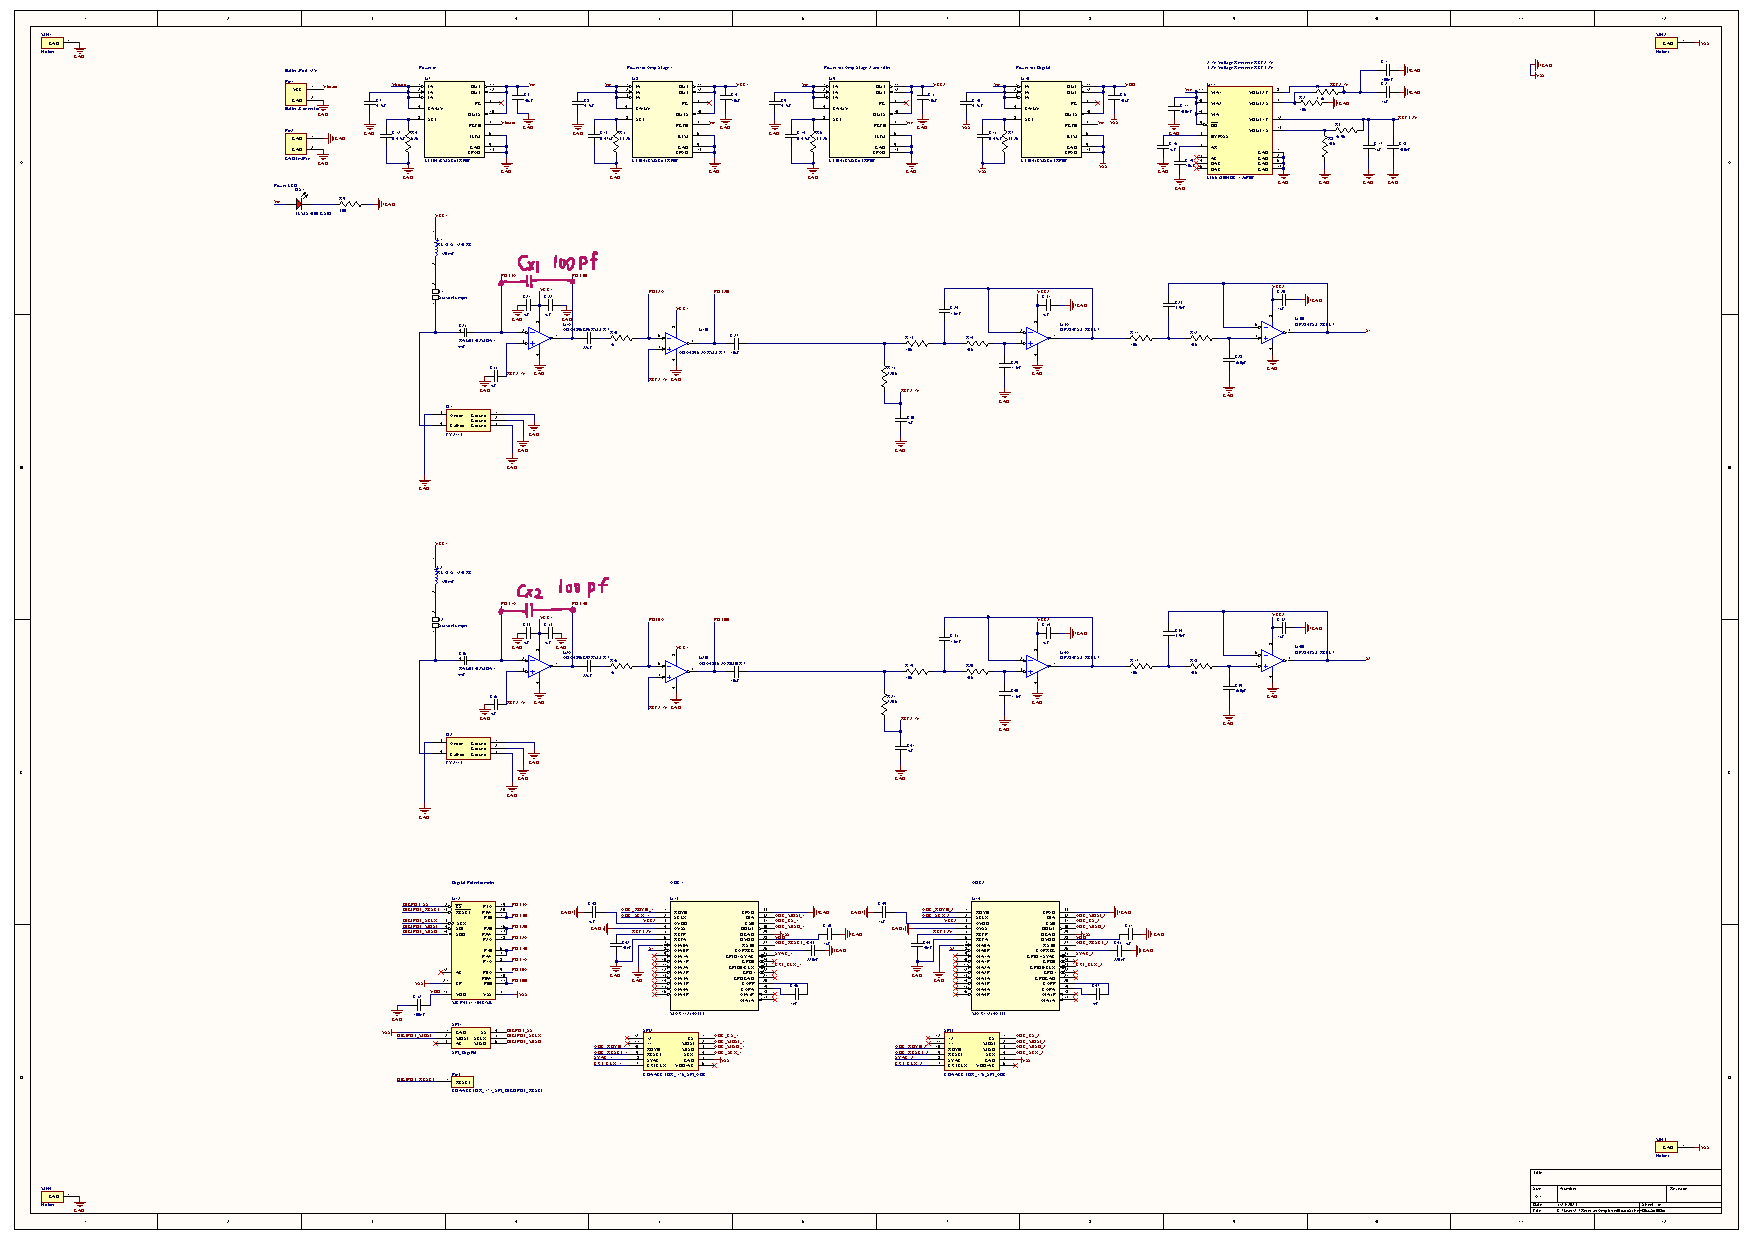
\includegraphics[width=1\linewidth]{4-ANC_Sys/ReceiverAmplifierBoardSchematic_23_5_2023.pdf}
\caption{Receiver Board Schematic}
\label{fig_sch}
\end{figure}

Fig.~\ref{fig_ReceiverBoard} and Fig.~\ref{fig_sch} depict the actual light receiver board together with the schematic of the light receiver board.  The PCB is designed using Altium Designer and manufactured at JLCPCB.

The receiver board has two stages of power supplies.  The first stage Low-dropout (LDO) regulator (LT3045EMSE) converts an externally supplied voltage within a range of~\qty{7}{V} to~\qty{20}{V} down to \qty{6.2}{V}.  To reduce interference and noise on the board, there are three second-stage LDOs (LT3045EMSE), two for analogue supply and one for digital supply, that all convert \qty{6.2}{V} to \qty{3.3}{V}.

Light reflected by the optrode consists mainly of background (DC component) light while the neural signal appears as a small (typically less than 10\% in amplitude) perturbation (AC component). Since only the biopotential signal part of the reflected light is of interest, and that the signal needs to be amplified at least 120dB to outperform the previous board, the DC part of the light must be removed before amplification.  Therefore, the amplifiers are AC coupled via a large capacitor right after the photodiode. When the photodiode is configured in reverse-bias, the system suffers from large $1/f$ noise that comes from the LDO. Therefore, the photo-diode D1 is configured in ``zero-mode''~\cite{zero-mode_detection}.  In this mode, the sensitivity is reduced because of the absence of DC biasing, but the noise from the DC biasing power supply is also removed, which makes the overall signal-to-noise ratio advantageous.

Fig.~\ref{fig_ReceiverSch} shows one channel of the final circuit schematic of the receiver board.  Compared to the schematic in Altium Designer, it adds a capacitor $C3$ and the photodiode is configured to zero mode, which reason will be discussed later.

\begin{figure}[h]
\centerline{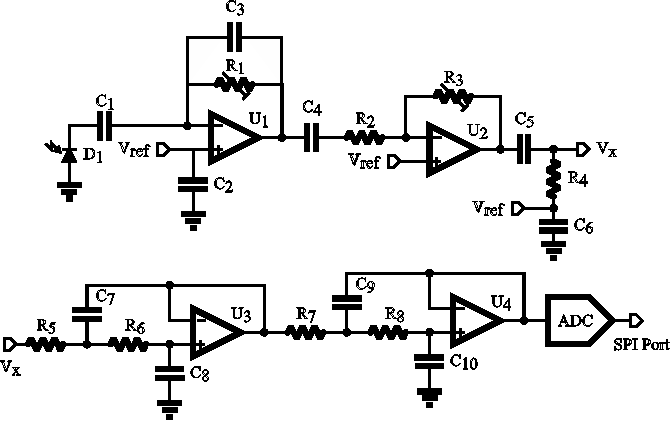
\includegraphics[scale=0.8]{4-ANC_Sys/ReceiverSch.pdf}}
\caption{Schmatic for one channel on light receiver board.  The upper half is a photodiode and a two-stage amplifier, and the bottom half is a two-stage low-pass-filter and an ADC.}
\label{fig_ReceiverSch}
\end{figure}

In fig.~\ref{fig_ReceiverSch}, $U_1$ and $U_2$ (ADA4896) are two stages of amplifiers.  A large capacitor $C_1$ makes sure only AC current is sent to op-amp $U_1$, which is configured as a transimpedance amplifier.  The gain of the transimpedance amplifier is set by a variable resistor $R_1$.  Op-amp $U_2$ along with $R_2$ and $R_3$ forms an inverting amplifier and the gain is controlled by variable resistor $R_3$.  The resistance of $R_1$ and $R_3$ both come from a digital potentiometer with  lowest resistance of \qty{390}{\Omega} and largest of~\qty{10000}{k\Omega}, which gives the two-stage amplifier a total gain from \qty{43.6}{dB\Omega} to \qty{140}{dB\Omega}.  The op-amps $U_1$ and $U_2$ are chosen to have very low noise, they have an input-referred voltage noise of~\qty{2.3}{nV/\sqrthz} and an input-referred current noise of~\qty{11}{pA/\sqrthz} at \qty{10}{\Hz}.  However, they also introduce~\qty{-11}{\mu A} input bias current, which is undesirable when dealing with large gains.  With $R_1$ set to \qty{10000}{k\Omega}, \qty{-11}{\mu A} input bias current will result in~\qty{-1.1}{V} output voltage. Therefore, Vref is set to be~\qty{2.1}{V} to have about~\qty{2}{V} peak-to-peak signal range and also~\qty{1.1}{V} bottom gap room.  The maximum input current from the photo-diode is~$\qty{2}{V}/\qty{140}{dB\Omega}=\qty{200}{nA}$.

The output voltage $V_x$ from the two-stage amplifier is then put through an active fourth-order anti-aliasing low-pass filter, consisting of $U_3$ and $U_4$ (LT6233).  The cut-off frequency is set to~\qty{13}{kHz} for the balance of the remaining signal up to \qty{10}{kHz} and anti-aliasing at ADC sampling frequency of \qty{64}{kHz}. Finally, a~\qty{24}{bit} \qty{64}{kHz} analogue to digital converter (MAX11254) converts the amplified analogue signal into a digital signal and is sent to the FPGA board (Arty Z7) via an SPI port.

A LTspice simulation of the light receiver board circuit is done to verify the circuit as shown in fig.~\ref{fig_LTspiceSim1} and fig.~\ref{fig_LTspiceSim2}.  Fig.~\ref{fig_LTspiceSim1} (a) and (b) show the circuit schematic of the two-stage amplifier and the simulation result of it.  A DC current source I1 and an AC current source I2 are used to simulate the behaviour of the photodiode since it is not included in the LTspice library and the manufacturer did not provide any simulation model.  The reverse-bias configuration is used here as it is the more conventional approach.  The rest of the circuits here are the same as the amplifier circuit in the PCB schematic.  Result shows that at \qty{10}{Hz} to \qty{10}{kHz}, the gain is constantly \qty{140}{dB\Omega}, and the lower \qty{3}{dB} frequency is at \qty{7.48}{Hz}, which is caused by the large AC coupling capacitor $C8$.  Fig.~\ref{fig_LTspiceSim2} (a) and (b) show the circuit schematic of the two-stage low-pass-filter and the simulation result of it.  The cut-off frequency is \qty{10.96}{kHz}, with a \qty{80}{dB} per decade roll-off, which matches the resistor and capacitor setting in the two-stage fourth-order active filter.  At the ADC working frequency \qty{64}{kHz}, the filter output is at \qty{-61.68}{dB}, which is sufficient for preventing aliasing.  When combining the two circuits, the output will have a bandwidth of \qty{10.96}{kHz}, starting at \qty{7.48}{Hz} and finishing at \qty{10.96}{kHz}, which suits the required working frequency (\qty{10}{Hz} to \qty{10}{kHz}) of the light receiver board.

\begin{figure}
\centering
\begin{subfigure}{1\textwidth}
  \centering
  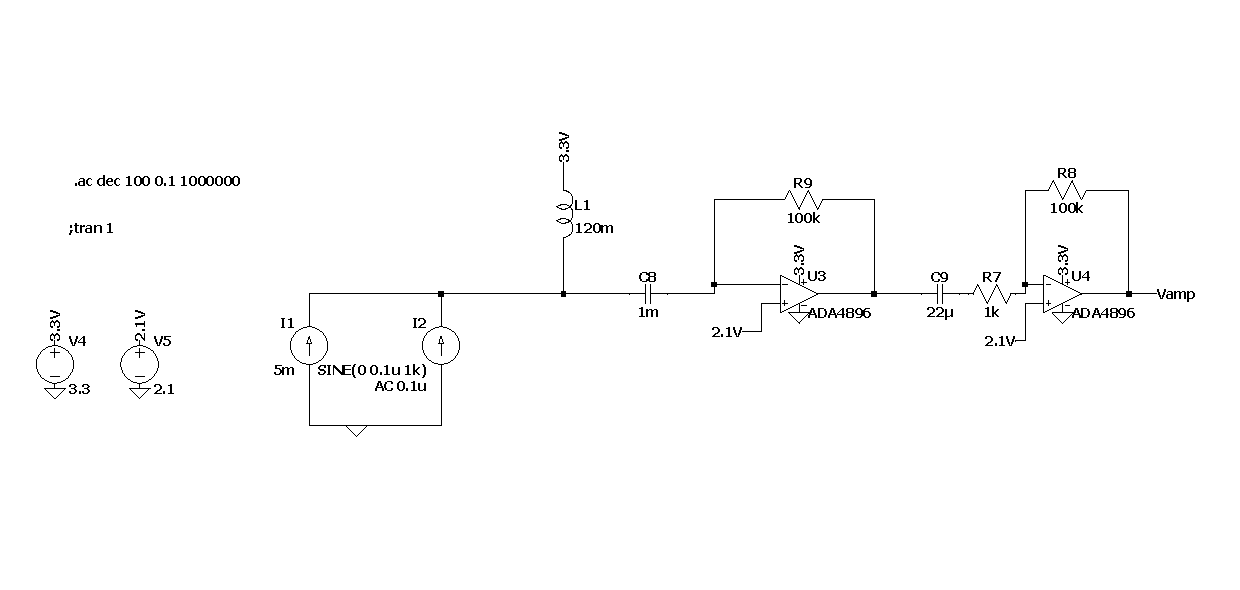
\includegraphics[width=1\linewidth]{4-ANC_Sys/LTspiceAmpSch.pdf}
  \caption{}
  \label{fig_LTspiceAmpSch}
\end{subfigure}
\begin{subfigure}{1\textwidth}
  \centering
  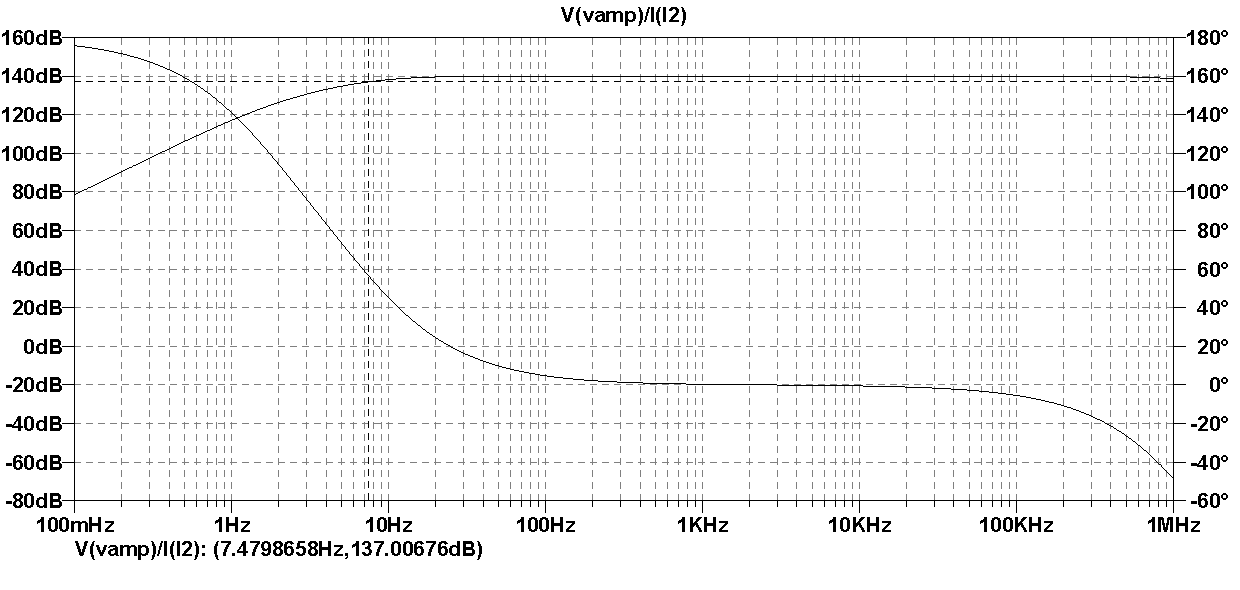
\includegraphics[width=1\linewidth]{4-ANC_Sys/LTspiceAmp.pdf}
  \caption{}
  \label{fig_LTspiceAmp}
\end{subfigure}
\caption{LTspice simulation on the light receiver circuit (a)Two-stage amplifier (b)Simulation result for amplifier}
\label{fig_LTspiceSim1}
\end{figure}

\begin{figure}
\centering
\begin{subfigure}{1\textwidth}
  \centering
  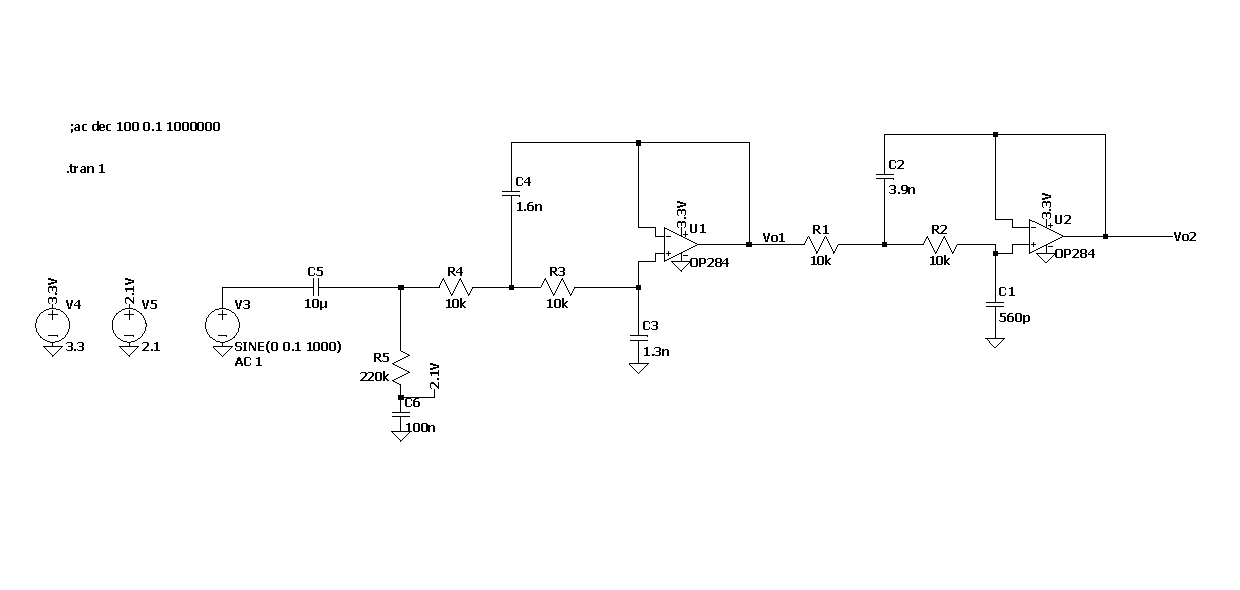
\includegraphics[width=1\linewidth]{4-ANC_Sys/LTspiceLPFSch.pdf}
  \caption{}
  \label{fig_LTspiceLPFSch}
\end{subfigure}
\begin{subfigure}{1\textwidth}
  \centering
  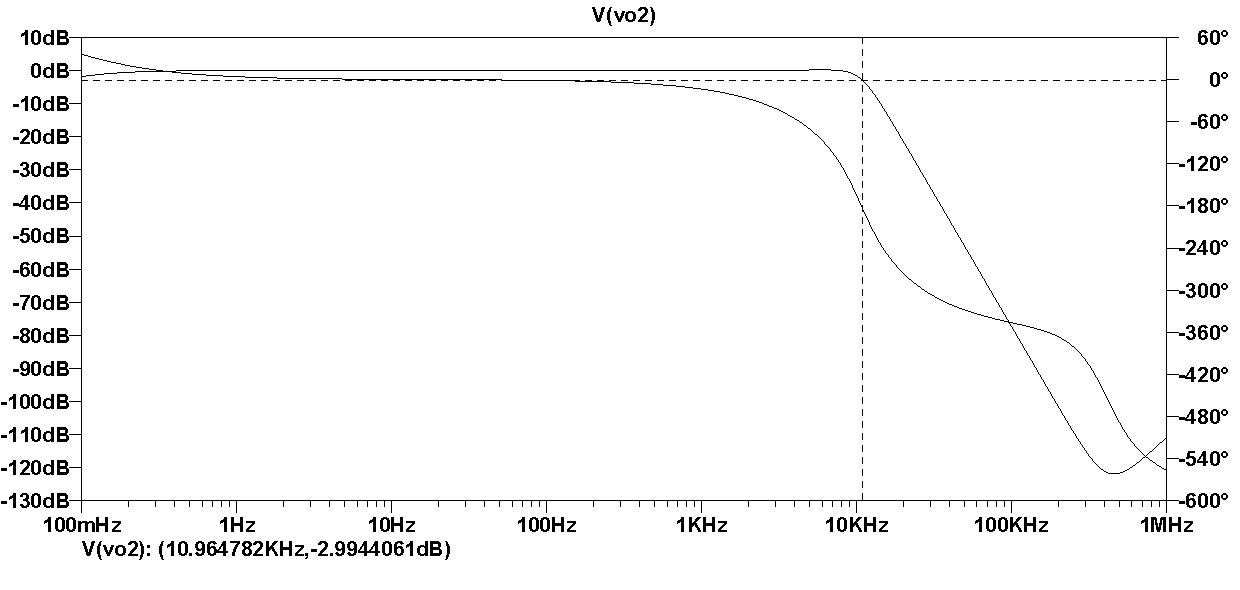
\includegraphics[width=1\linewidth]{4-ANC_Sys/LTspiceLPF.pdf}
  \caption{}
  \label{fig_LTspiceLPF}
\end{subfigure}
\caption{LTspice simulation on the light receiver circuit (a)Two-stage low-pass-filter (b)Simulation result for filter}
\label{fig_LTspiceSim2}
\end{figure}

\begin{figure}[H]
\centering
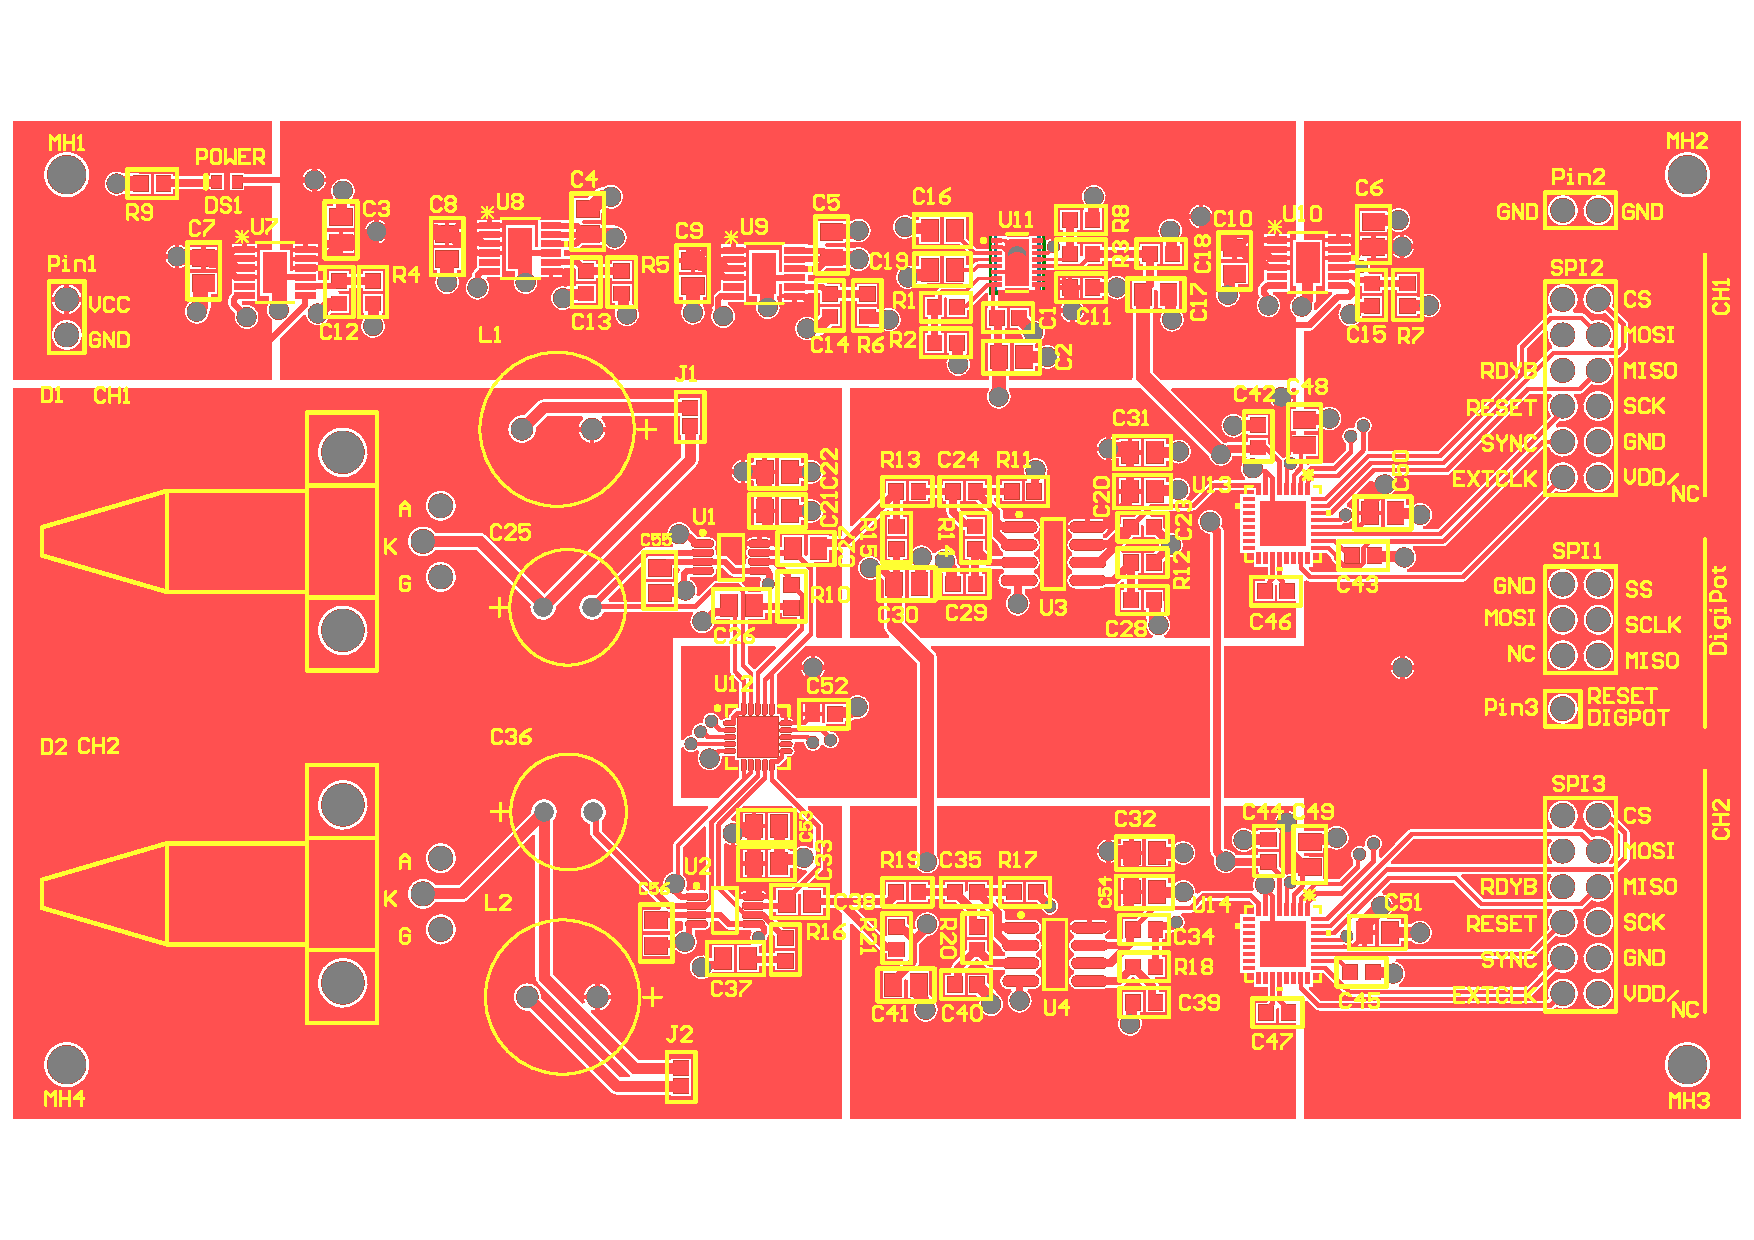
\includegraphics[width=0.9\linewidth]{4-ANC_Sys/PCB.pdf}
\caption{Receiver Board PCB Design top layer}
\label{fig_PCB}
\end{figure}

\begin{figure}[H]
\centering
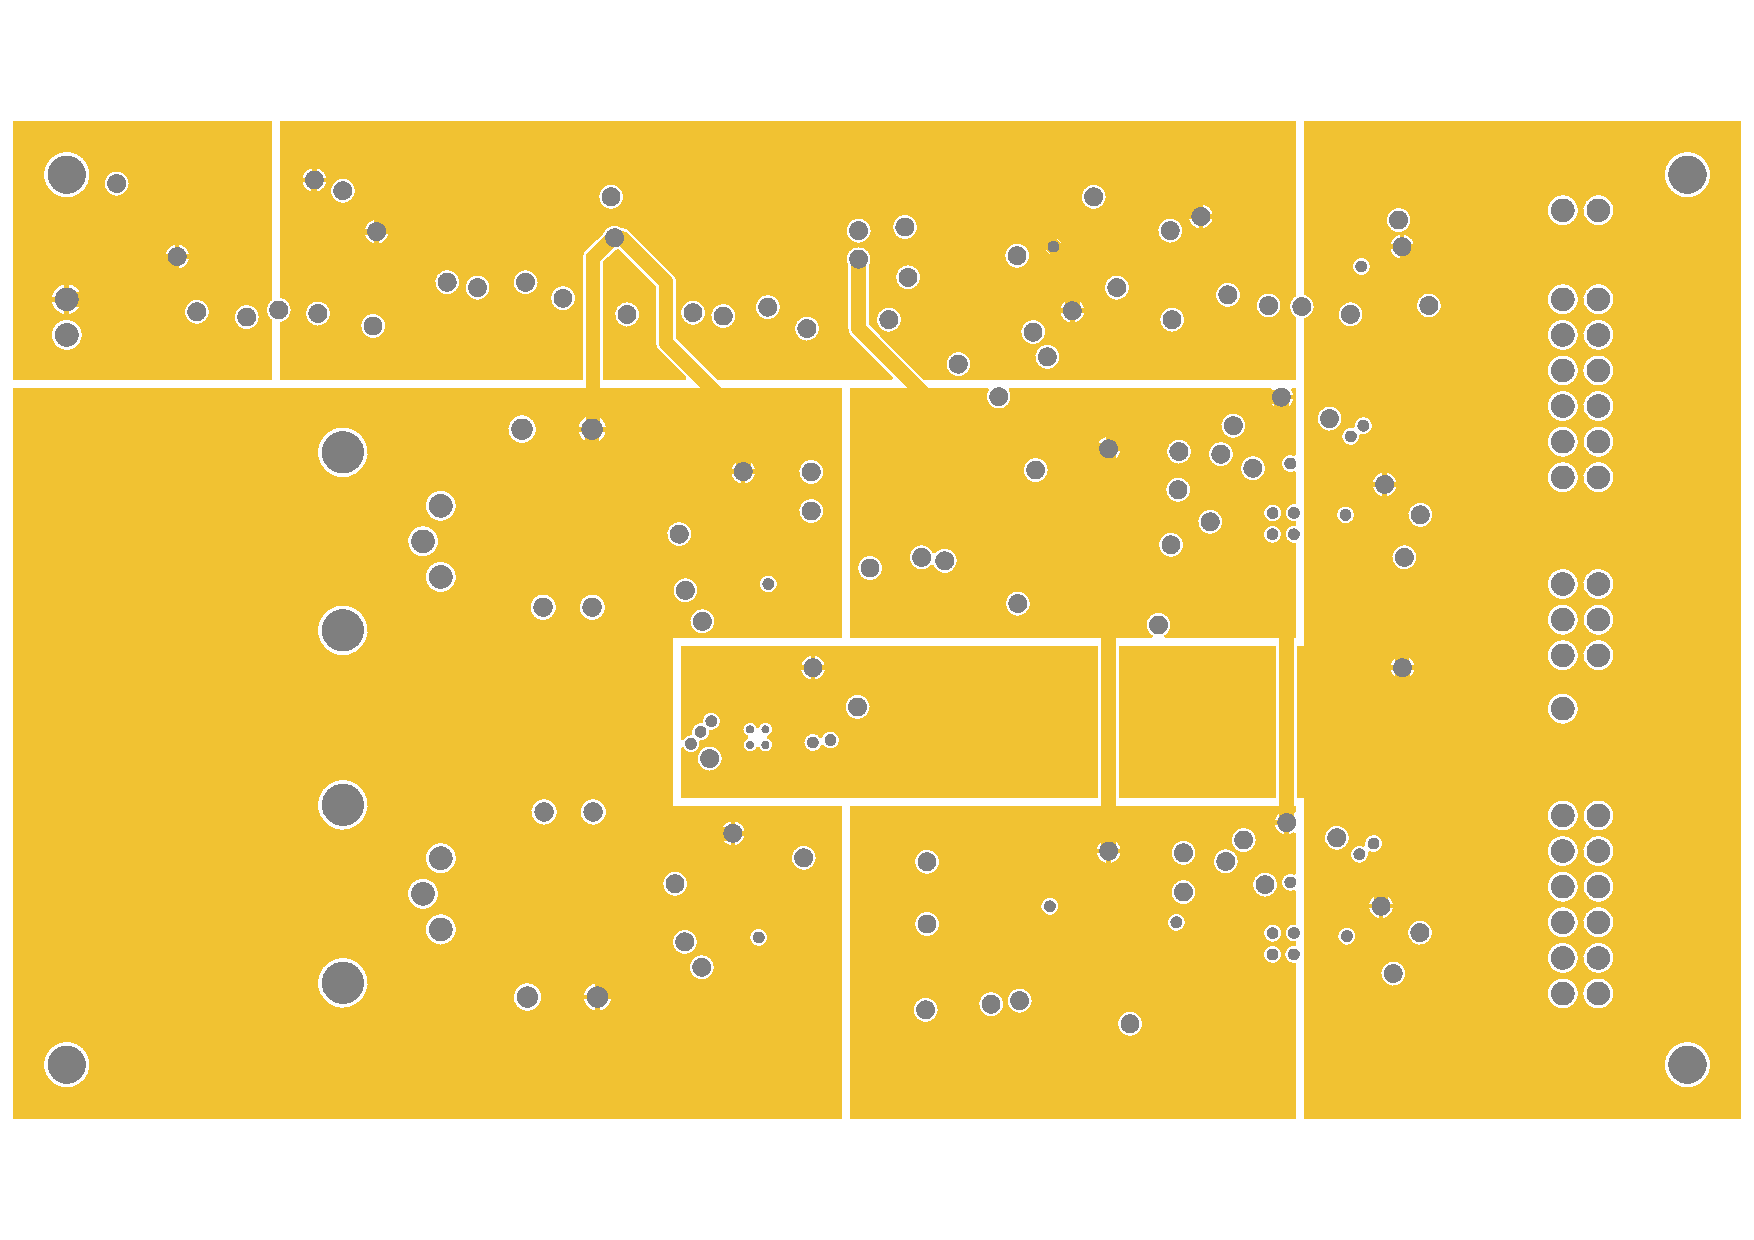
\includegraphics[width=0.9\linewidth]{4-ANC_Sys/PCB_2.pdf}
\caption{Receiver Board PCB Design power layer}
\label{fig_PCB_2}
\end{figure}

\begin{figure}[H]
\centering
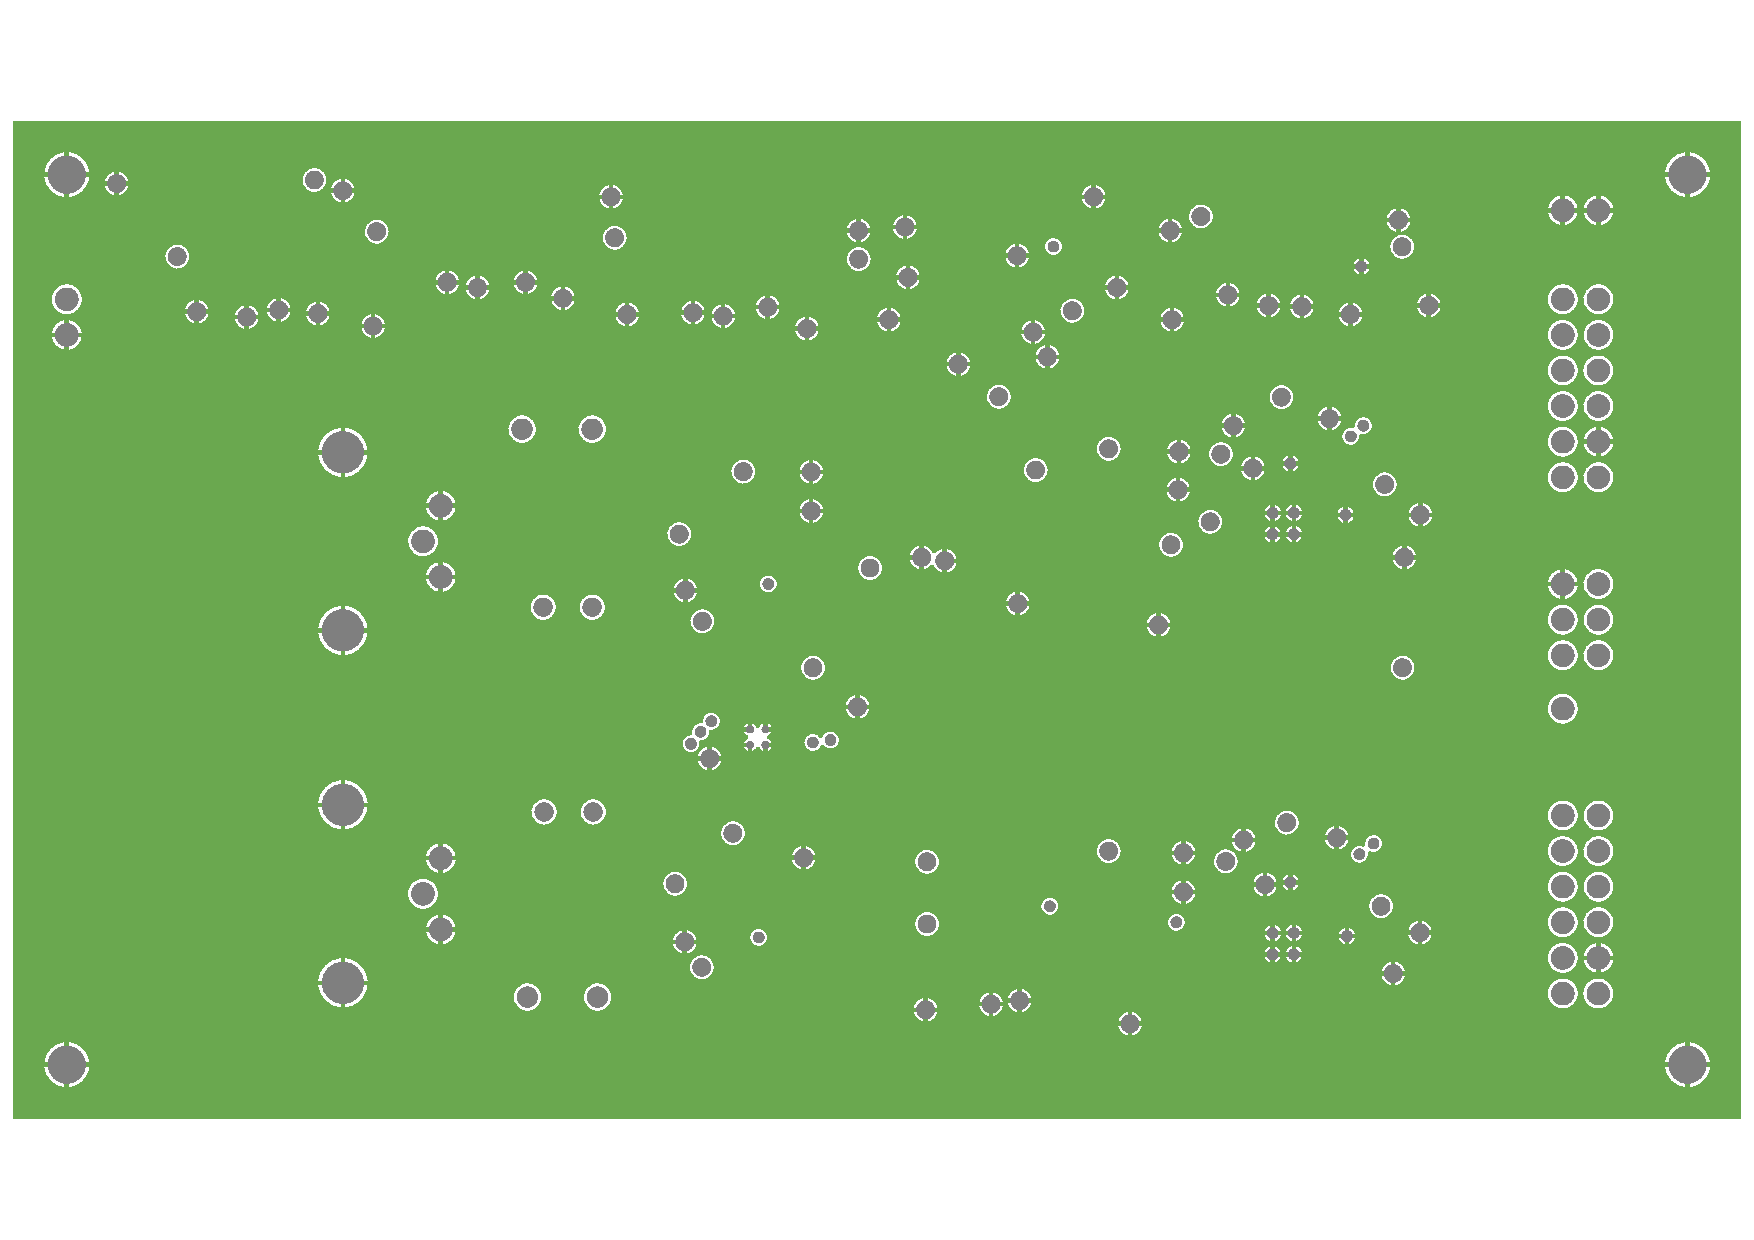
\includegraphics[width=0.9\linewidth]{4-ANC_Sys/PCB_3.pdf}
\caption{Receiver Board PCB Design ground layer}
\label{fig_PCB_3}
\end{figure}

\begin{figure}[H]
\centering
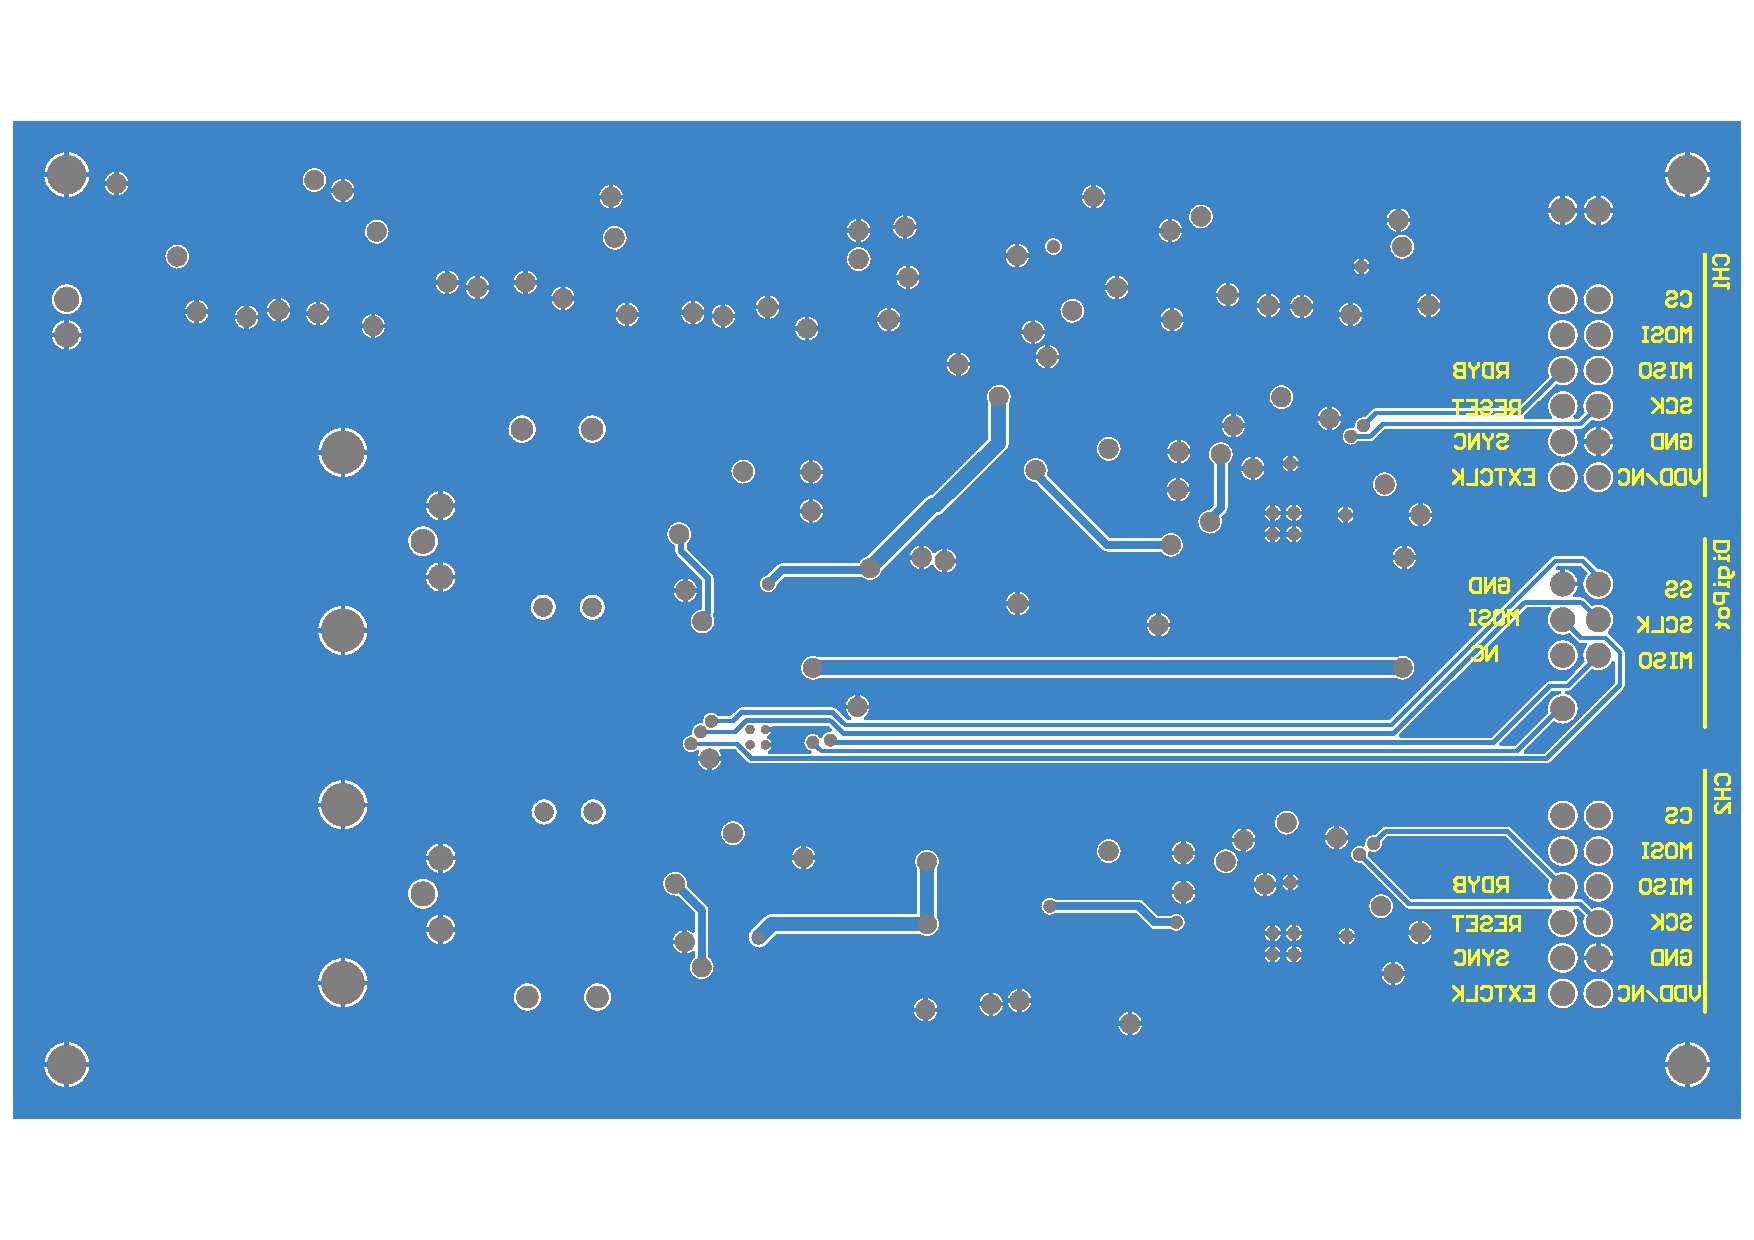
\includegraphics[width=0.9\linewidth]{4-ANC_Sys/PCB_4.pdf}
\caption{Receiver Board PCB Design bottom layer}
\label{fig_PCB_4}
\end{figure}


Fig.~\ref{fig_PCB} to fig.~\ref{fig_PCB_4} shows the PCB layout of the light receiver board.  It is a four-layer design with two power layers and two signal layers.  Fig.~\ref{fig_PCB} shows the top layer of the PCB, which is the layer where most of the components are mounted.  Most of the signal tracks also goes through this layer to connect all the components.  Fig.~\ref{fig_PCB_2} shows the power layer, that provides power supply to most of the components.  It has five planes for five different power supplies.  The plane on the top left is the input power plane, this plane is connected to the external power source.  The plane at the center top is the $V_{in}$ plane, which is the output of the first stage LDO.  The bottom left plane is one of the analogue \qty{3.3}{V} supply plane, the light to current converting and amplifying happens in this plane. The plane at upper middle and the plane at the middle bottom are connected together, and they are the second analogue \qty{3.3}{V} plane, that powers the active filters and analogue side of the ADC.  The plane at lower middle and at far right is the digital supply.  The digital plane powers the digital potentiometer and the digital side of the two ADCs.  The top layer also has the same planes for better power transmission.  The third layer shown in fig.~\ref{fig_PCB_3} is the ground layer.  This layer has one large plane that covers the whole board and provide good ground connections to all the components.  The bottom layer shown in fig.~\ref{fig_PCB_4} lays the signal tracks that can not be fitted in the top layer, and is also covered by a large ground plane.

$Pin1$ is the power pin that connects to a voltage source at a range of \qty{7}{V} to \qty{20}{V}, and passes the voltage to $U7$, which is the first stage of LDO.  The output of $U7$ is \qty{6.2}{V}, and that powers a power indicator LED $DS1$, three second stage LDOs $U8$, $U9$, and $U10$, and a voltage reference $U11$.  LDO $U8$ powers the reverse biasing circuit for the photodiode and the two stages of amplifier $U1$ and $U2$ for both channels.  LDO $U9$ powers the two-stage active filters $U3$ and $U4$ for both channels.  LDO $U10$ powers ADCs $U13$ and $U14$, and the digital potentiometer $U12$.  Voltage reference $U11$ provides reference bias voltage for the amplifiers and reference voltage for the ADC.  All the power chips are located on the top of the board.  Channel 1 and channel 2 are at the middle and bottom of the board.  For each channel, from left to right lays the photodiode, reverse bias inductor, AC couple capacitor, two stages of amplifier, two stages of low pass filter, analogue digital converter, and digital output pins.  The digital potentiometer is located between the amplifiers for the two channels, for lower interference.  Chips are placed within their corresponding power planes for lower electromagnetic interference, better power stability, and less loop area.  $J1$ and $J2$ are designed to be "switches`` to convert the configuration between reverse bias and zero-mode for the photodiode.  $Pin2$ on the top right of the board provides a ground point for testing.  All the output pins are \qty{2.54}{mm} pitch connectors for easier cable making.


\subsection{New light receiver board testing}

The new receiver board PCB is manufactured at JLCPCB.  Tests for the board performance are done after all the components are soldered up.  A stability issue is found right after we start testing, the amplifier is unstable at the whole required working frequency range.   This problem is solved by adding a \qty{100}{pF} capacitor across the first stage of the amplifier as shown as $C5$ in fig.~\ref{fig_ReceiverSch}.  This issue could be caused by inductance created by the track on the PCB board, however, we do not have time to investigate more on that.  Since the capacitor fixed the issue, we moved on to the next test.

\begin{figure}[h]
\centerline{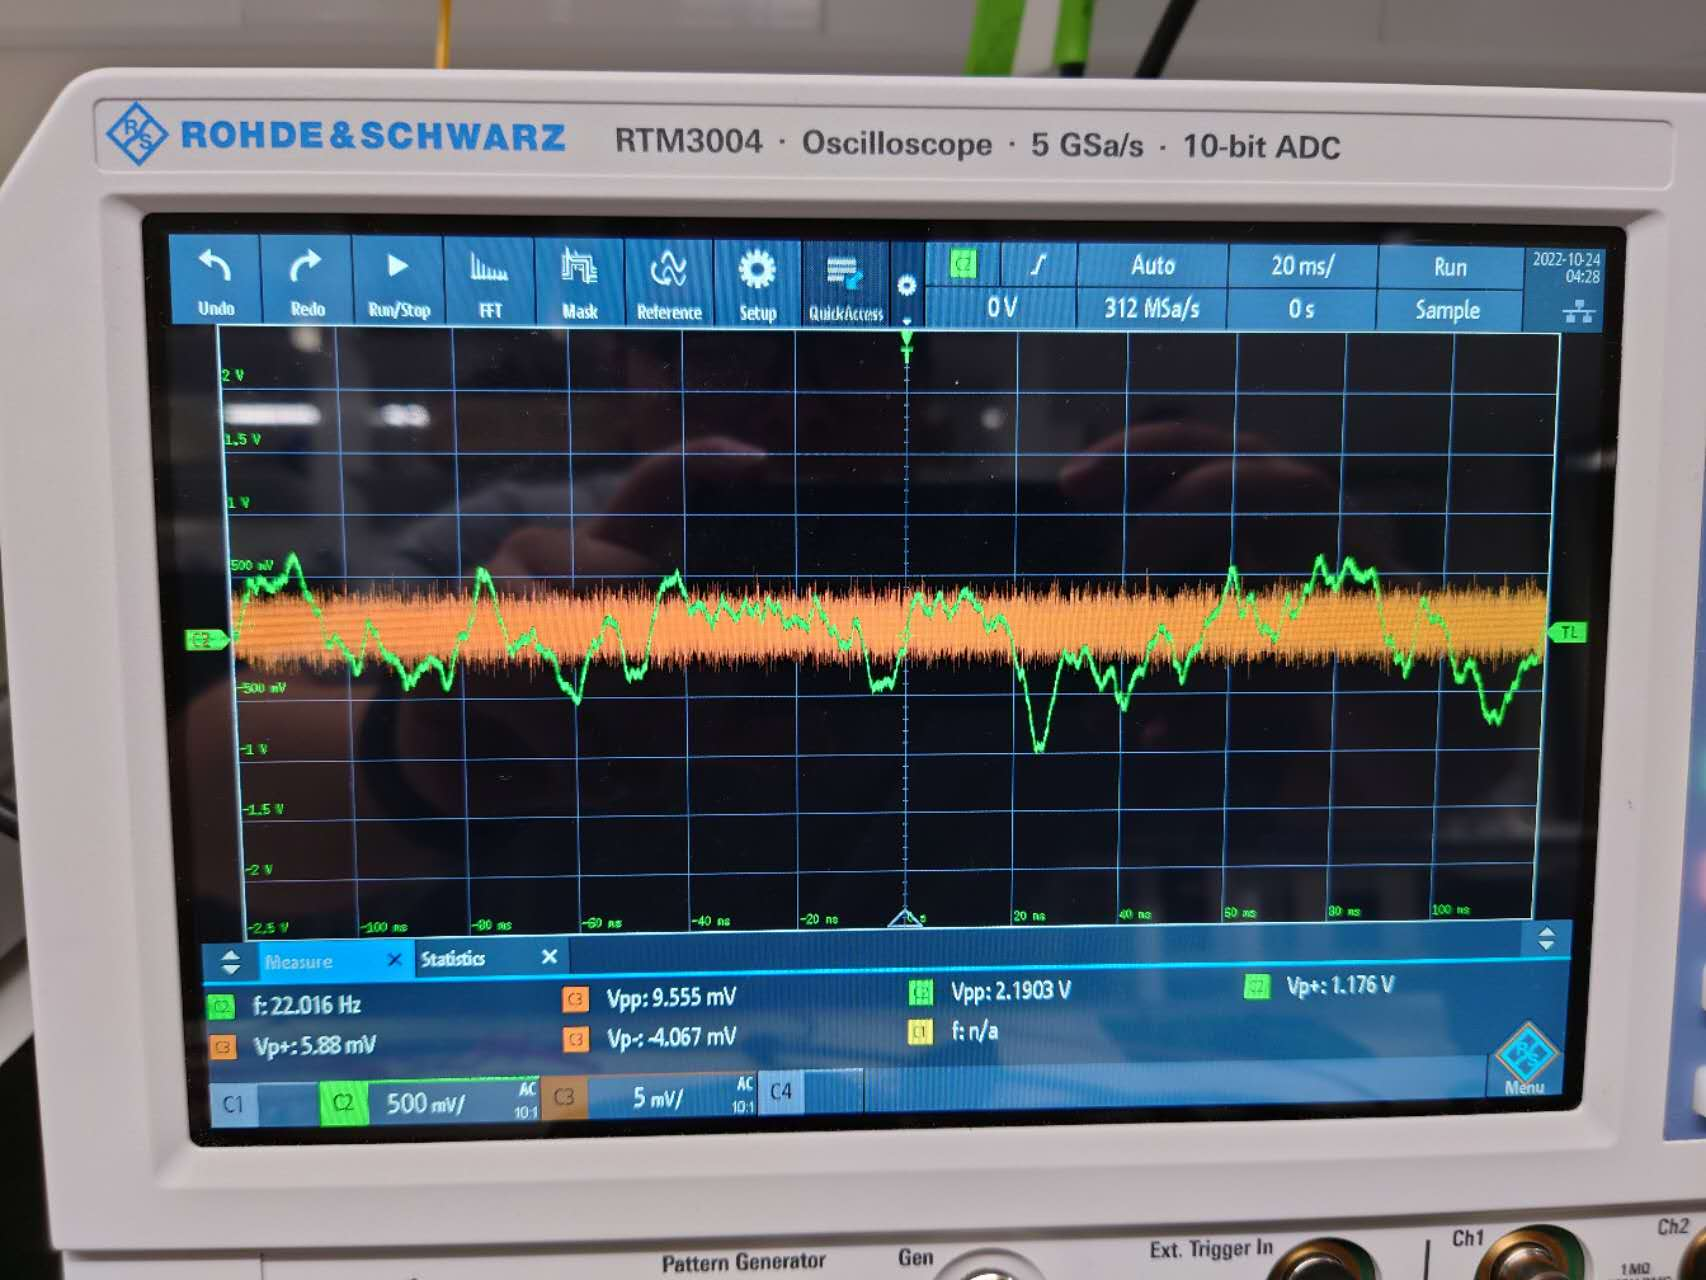
\includegraphics[width=1\linewidth]{4-ANC_Sys/LargeNoiseRecBoard.jpg}}
\caption{Receiver board input and output at \qty{140}{dB\Omega}, zero input, output shows very large $1/f$ noise.}
\label{fig_ReceiverBoardLargeNoise}
\end{figure}

Tests are done for the new light receiver board with the photodiode configured as reverse-biased first since this is the conventional way.  The amplifier is working fine, as they have the correct output gain as set.  However, there is also very large noise (\qty{1}{V} peak-to-peak) at the output of the two-stage amplifier as shown in fig.~\ref{fig_ReceiverBoardLargeNoise}.  The noise here has the same amplitude as the largest designed signal output amplitude, which is unacceptable.  Then we change the photodiode configuration to zero mode, which in theory should generate less noise into the system.  The results show around \qty{5}{mV} peak-to-peak noise output, which is a lot less than the reverse-bias configuration.  Fig.~\ref{fig_RecBoardNoiseTest} shows the current noise at the input of the first stage amplifier, which the data is converted back from the output voltage noise measurement, using the gain parameter of \qty{140}{dB\Omega}.  The reverse-bias photodiode configuration shown in fig.~\ref{fig_NoiseReverseBias} generates a lot of $1/f$ noise than the zero mode configuration shown in fig.~\ref{fig_NoiseZeroMode}.  To find out what caused the noise performance difference, we have looked into the circuit schematic.  The reverse-bias configuration has one more connection to a bias inductor and is then connected to the \qty{3.3}{V} LDO power supply.  Since the inductor is a passive component, with a DC resistance of \qty{97}{\Omega}, it does not generate a lot of noise.  The LDO on the other hand, generates up to \qty{100}{nV/\sqrthz} voltage noise at \qty{10}{Hz}, and reduces to and stays at \qty{2}{nV/\sqrthz} at \qty{1}{kHz} and higher frequency.  If we convert this value to current noise using the \qty{97}{\Omega} resistance at the inductor, we get about \qty{1}{nA/\sqrthz} at \qty{10}{Hz} and about \qty{10}{pA/\sqrthz} at \qty{1}{kHz}.  This is slightly larger than the value in fig.~\ref{fig_NoiseReverseBias}, but still matches very well.  The zero mode noise, although also slightly smaller than the datasheet value, also matches the value on the amplifier (ADA4896) value quite well.  Therefore, zero mode configuration is the better choice in this case, as it generates a lot less noise than the reverse-bias mode because there is one less noise source (LDO).


\begin{figure}[h]
\centering
\begin{subfigure}{.5\textwidth}
  \centering
  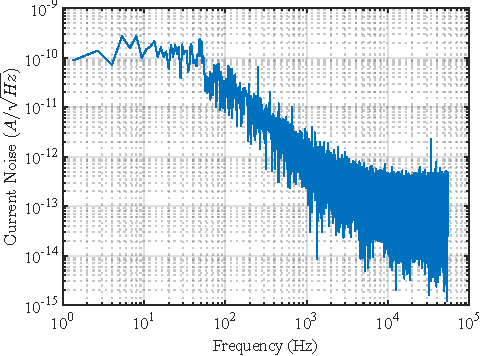
\includegraphics[width=1\linewidth]{4-ANC_Sys/NoiseReverseBias.pdf}
  \caption{}
  \label{fig_NoiseReverseBias}
\end{subfigure}%
\begin{subfigure}{.5\textwidth}
  \centering
  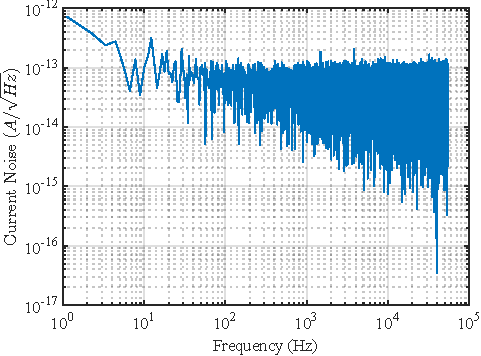
\includegraphics[width=1\linewidth]{4-ANC_Sys/NoiseZeroMode.pdf}
  \caption{}
  \label{fig_NoiseZeroMode}
\end{subfigure}
\caption{Light receiver board noise test with floating input (a) Reverse-bias photodiode (b) Zero mode}
\label{fig_RecBoardNoiseTest}
\end{figure}

Further testing on gain and bandwidth is made to only the zero mode configuration since it will not be practical to test and use reverse-bias configuration because of the large noise.  Before testing the board with the light circuit, we first test it with electrical input.  Fig.~\ref{fig_BoardTest1khz} shows the input and output waveform when testing the new light receiver board.  The input is a \qty{23}{mV} \qty{1}{kHz} sinusoidal signal connected to the point between the photodiode and the AC coupling capacitor, via a \qty{100}{k\Omega} resistor.  This is because the photodiode outputs current, and so we need a resistor to convert the voltage input into current input.  The output is measured at the output of the two-stage low-pass filter.  From this output voltage, the gain can be calculated as:
$$Gain=\frac{V_{out}}{I_{in}}=\frac{V_{out}}{\frac{V_{in}}{R_{in}}}=\frac{\qty{1.8395}{V}}{\frac{\qty{23}{mV}}{\qty{100}{k\Omega}}}=\qty{138.06}{dB}$$

\begin{figure}[H]
\centering
\includegraphics[width=1\linewidth]{4-ANC_Sys/BoardTest1khz.png}
\caption{Board test at \qty{1}{kHz}}
\label{fig_BoardTest1khz}
\end{figure}

Fig.~\ref{fig_BoardBandwidth} shows the gain at a few more frequency points.  The gain at maximum setting is at \qty{138}{dB}, which is \qty{2}{dB} lower than the \qty{140}{dB} theoretical maximum gain.  This might be caused by resistor inaccuracy, PCB track resistance and interference, or measurement error.  Overall, \qty{2}{dB} error is acceptable.  The \qty{3}{dB} bandwidth is basically the same as the simulation result, with the lower \qty{3}{dB} point at just under \qty{10}{Hz}, and the higher \qty{3}{dB} at just over \qty{10}{kHz}.  This result confirms the board is working as expected, and it meets the frequency requirement of the optrode system.

\begin{figure}[H]
\centering
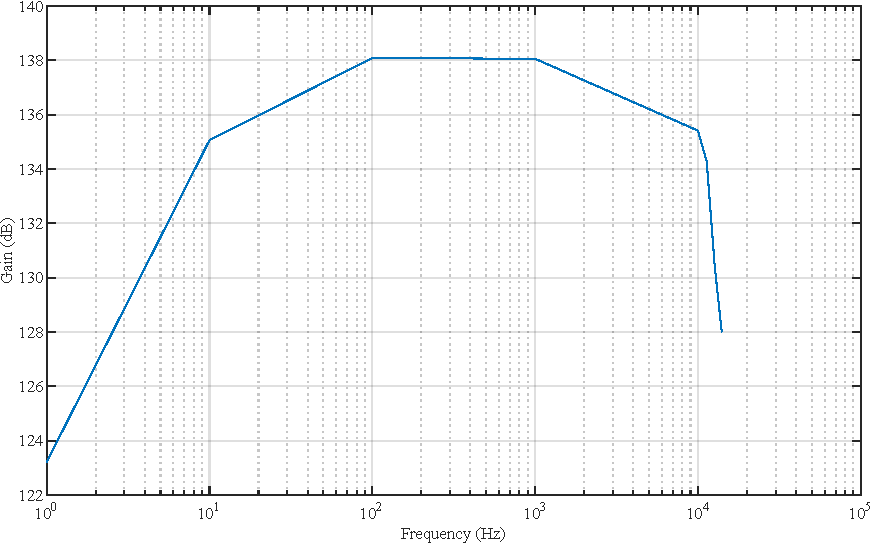
\includegraphics[width=1\linewidth]{4-ANC_Sys/BoardBandwidth.pdf}
\caption{Board bandwidth test}
\label{fig_BoardBandwidth}
\end{figure}




\section{Development of the noise cancelling algorithm}

\subsection{Wiener filter}

An effective noise cancelling algorithm is essential for the active noise cancelling concept to work in the optrode system.  What we want is an algorithm that is not too complex, can handle real-time input-output, and is easy to scale up to hundreds of channels.  One of the common methods for active noise cancelling is the wiener filter.  eqn~\ref{eqn_WienerMatrix} from the literature review shows how to perform the calculation for the wiener filter.  In this equation, matrix $T$ contains a symmetric Toeplitz matrix of $R_w$, which is the autocorrelation of the signal $w$.  Matrix $a$ contains the filter coefficient $a$, and matrix $v$ contains $R_{ws}$, which is the cross-correlation of the signal $w$ and the signal $s$.  We know the information in the signal $w$ and $s$, so we can calculate $R_w$ and $R_{ws}$, therefore also matrix $T$ and $v$ using the following equation:
$$R_w[m]=E\{w[n]w[n+m]\}$$
$$R_{ws}[m]=E\{w[n]s[n+m]\}$$
Where $E$ denotes the expectation operator.

From these equations, we can write code to generate filter coefficients.  However, this method uses the whole length of $w$ and $s$ and the generated coefficient $a$ has the same length.  This process takes a very long time and a lot of computational resources.  From the testing result in fig.~\ref{fig_CrossCorrelationTest}, we can see that the signals are only largely correlated at 7 samples, which means there are not a lot of similarities between the two signals beyond 7 samples and we should be able to use fewer filter coefficients and achieve similar performance as the whole data length filter coefficients.  Below is a MATLAB code for a modified wiener filter function, the input is two signals $x$ and $y$, the number of filter taps, and the number of samples shifted between $x$ and $y$.  The output is $xest$ the estimated x and $FilterVector$ the filter coefficients.

\begin{lstlisting}[language=matlab]
function [FilterVector,xest] = myWiener(x,y,N,NS)
%
% Wiener filter based on Wiener-Hopf equations
%   This function takes as inputs a noisy signal, x, and a reference signal, y,
%   in order to compute a N-order linear filter that provides an estimate of y
%   from x
%  
% INPUTS
% x = noise + message signal
% y = noise signal
% N = filter order
% Ns = filter shift
%
% OUTPUTS
% xest = estimated signal
% FilterVector = Wiener filter coefficients

% Autocorrelation function
for i = 1:length(x)
    Rxx(i) = 0;
    for j = 1:length(x)
        if i + j <= (length(x) + 1)
            Rxx(i) = Rxx(i) + x(j) * x(j+i-1);
        else
            Rxx(i) = Rxx(i) + x(j) * x(j+i-length(x)-1);
        end
    end
end
% Crosscorrelation function
for i = 1:length(x)
    Rxy(i) = 0;
    for j = 1:length(x)
        if i + j <= (length(x) + 1)
            Rxy(i) = Rxy(i) + x(j) * y(j+i-1);
        else
            Rxy(i) = Rxy(i) + x(j) * y(j+i-length(x)-1);
        end
    end
end
%

Rxx = toeplitz(Rxx);
Rxy = Rxy';
B = Rxx \ Rxy;

% Create filter window centered at 1
FilterVector = zeros(1,NS-floor(N/2));
WorkingFilter = (B(NS+1-floor(N/2):NS+1-floor(N/2)+N-1))';
FilterVector = cat(2, FilterVector, WorkingFilter);

xest = filter(FilterVector,1,x);
\end{lstlisting}

------------------------------
Originally from online, modified by myself.
------------------------------

Fig.~\ref{fig_TestMeasurement} shows the result of running the MATLAB code above on a set of biomedical data recorded previously.  The green $Detrend SOptrode$ is the channel that contains the cardiac signal captured with optrode, and the black $ Detrend SNoiseRef$ is the other channel that comes out from the same light source but not into an optrode.  Both of them are detrended because there has been a very slow DC level shifting because the data is captured before the capacitor on the previous receiver board has been charged up.  The red signal $Estimated Noise$ is the $Xest$ output from $myWiener$ function, and the blue signal is the green original signal subtracting the red estimated noise.  In this case, $myWiener$ function takes the input of optrode and noise reference signals and estimates a noise signal that correlates most to the optrode signal.  If we take a period of time in the flat part of the signal, i.e. from \qty{0.7}{s} to \qty{0.8}{s}, and compare the RMS value for the green and blue signal, which is the original and after process signal, we get around 30\% reduction rate.  


\begin{figure}[h]
\centering
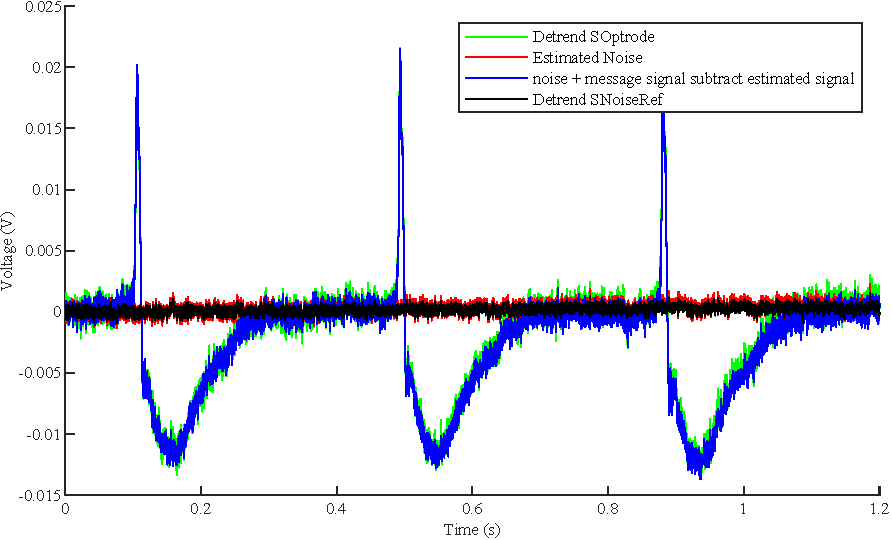
\includegraphics[width=1\linewidth]{4-ANC_Sys/TestMeasurement.pdf}
\caption{TestMeasurement}
\label{fig_TestMeasurement}
\end{figure}

\subsection{Modifing Wiener filetr}
Now we have a working algorithm, we need to figure out how to meet the other two requirements: real-time processing, and easy to implement on FPGA.  In order to take real-time digital input sample by sample, we cannot use the whole data set, and it is not very simple to implement a moving bin algorithm on the FPGA.  Therefore, we decided to use a leaky integrator, so the weighting for each sample is at maximum when it first comes in, and gradually reduces by 0.01\% per sample.  At this rate, reducing each sample to about 5\% of the original value will require 29956 samples, which would be \qty{3}{s} at \qty{10}{kHz} sampling rate in this model.  A high-pass filter is implemented to remove the effect of DC-level shifting.  The high-pass filter block has a transfer function of $H(z)=\frac{1-Z^{-1}}{1-0.9Z^{-1}}$, at \qty{10}{kHz} sampling frequency, the cut off frequency would be around \qty{151}{Hz}.  In eqn~\ref{eqn_WienerMatrix}, if we simplify the matrix to one sample length, the filter coefficient $a$ is given by the cross-correlation of $w$ and $s$ divided by the autocorrelation of $w$.  We perform a similar process here by multiplying $NoisySignal$ and $Noise$ and integrating to get the cross-correlation, and multiplying $Noise$ by itself and integrating to get the auto-correlation, then dividing the cross-correlation to the auto-correlation to get the filter coefficient.  We multiply the $Noise$ signal by this filter coefficient to get the estimated $Noise$ signal that best matches the noise in $NoisySignal$.  Finally, subtract $NoisySignal$ by the estimated $Noise$ to get the active noise cancelling output.  This modified wiener filter structure is constructed with Simulink and shown in fig.~\ref{fig_Simulink}.  The test result of this Simulink model using the same data input as the wiener filter test is shown in fig.~\ref{fig_SimulinkResult}.  The blue signal is $NoisySignal$ at the input and the green signal is the output of the Simulink model.  The improvement is very close to the wiener filter result in fig.~\ref{fig_TestMeasurement}, which proves this Simulink model is effective for reducing the noise in biomedical signals.

\begin{figure}[h]
\centering
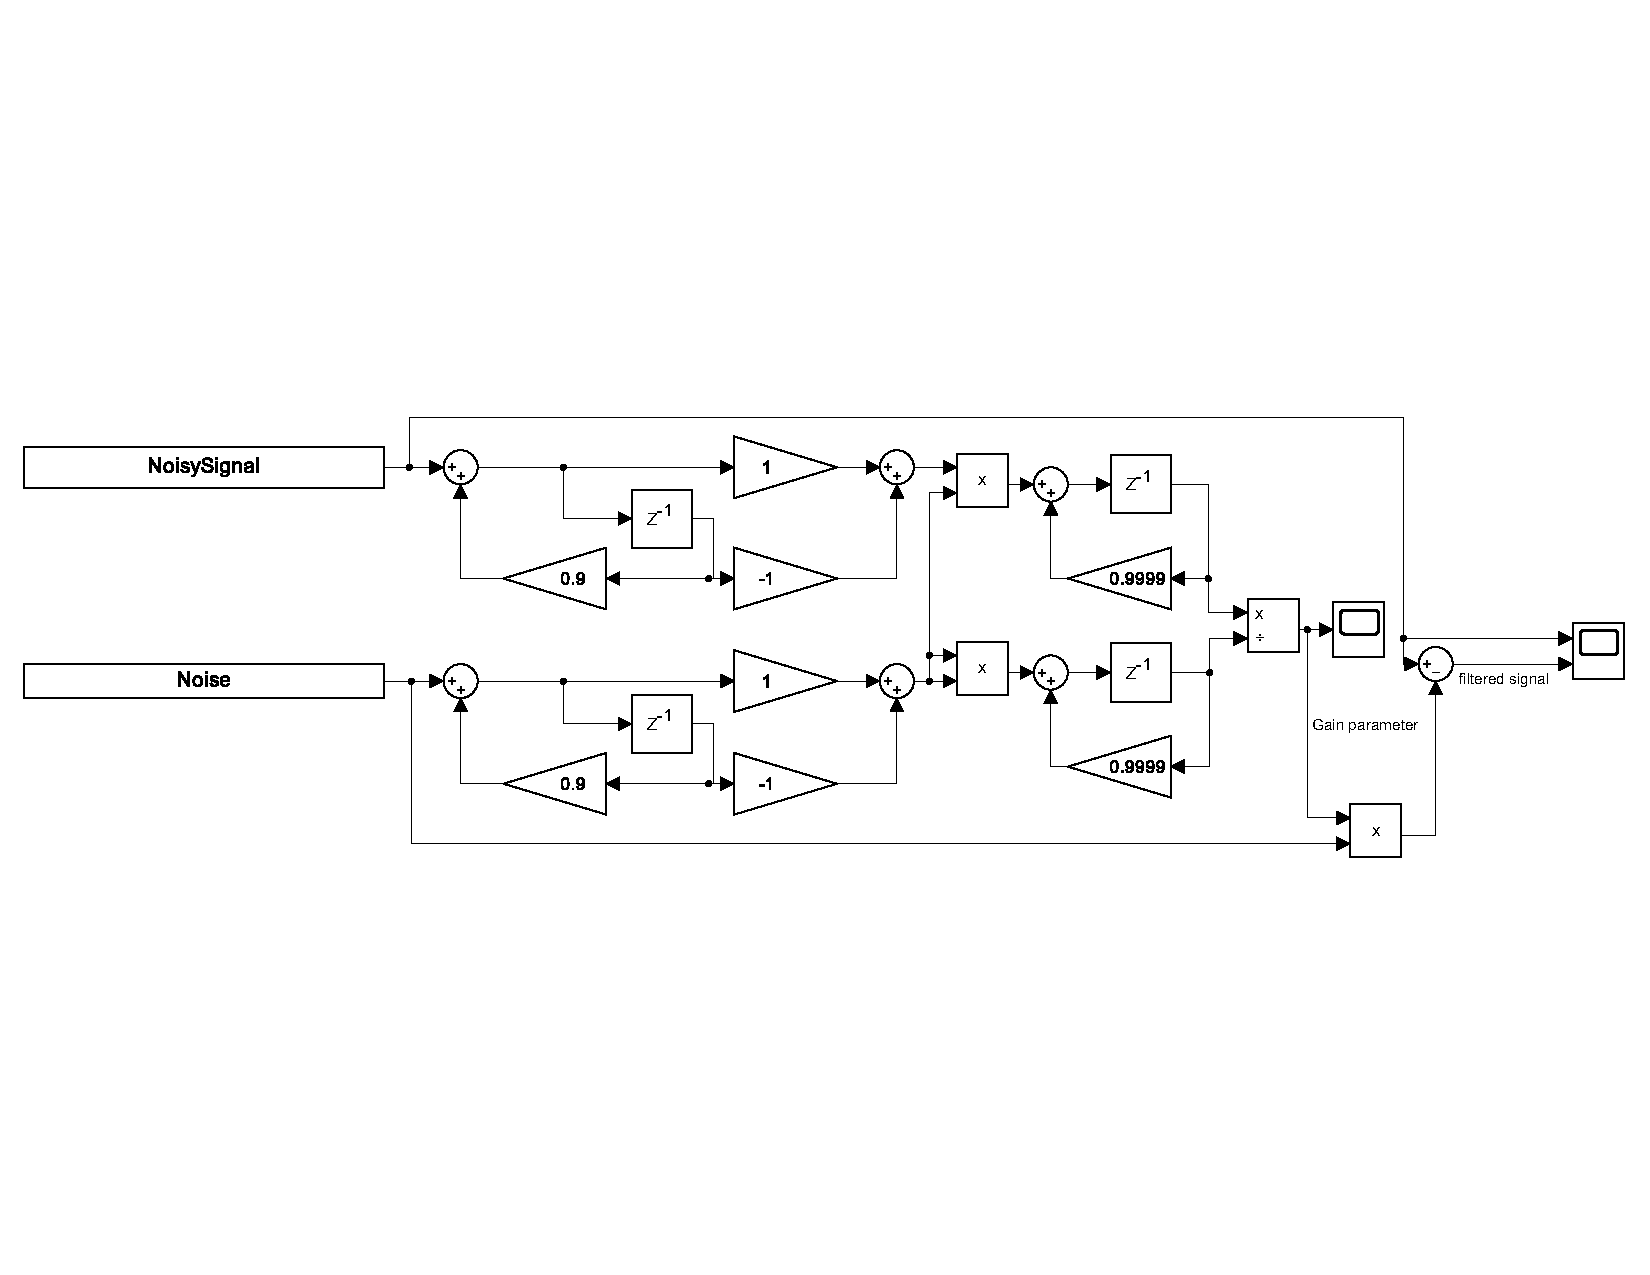
\includegraphics[width=1\linewidth]{4-ANC_Sys/Simulink.pdf}
\caption{Simulink DSP block}
\label{fig_Simulink}
\end{figure}

\begin{figure}[h]
\centering
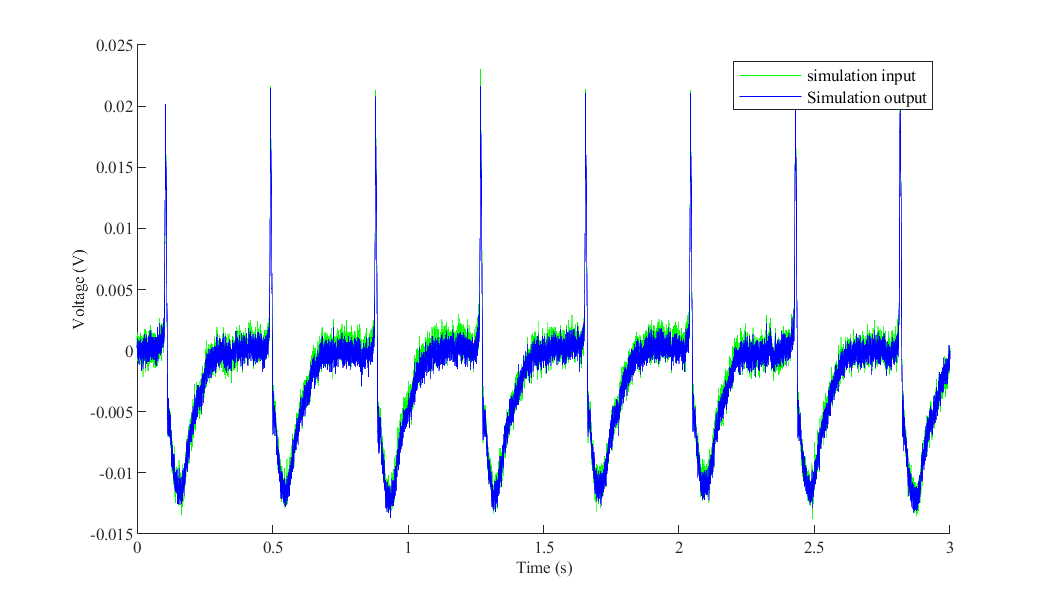
\includegraphics[width=1\linewidth]{4-ANC_Sys/SimulinkResult.pdf}
\caption{Simulink DSP Result}
\label{fig_SimulinkResult}
\end{figure}

\subsection{Verilog HDL implementation}

Fig.~\ref{fig_VivadoBD_DSP} and fig.~\ref{fig_VivadoSimResult} show the simulation in Xilinx Vivado of the Simulink model discussed above.  The purpose of this simulation is to modify and confirm the Simulink model can work on an FPGA.  Fig.~\ref{fig_VivadoBD_DSP} shows a register-transfer level (RTL) DSP model written in Verilog HDL, which can be run on the FPGA in real-time.  Small operation blocks are made similar to Simulink blocks, so the block diagram DSP structure looks the same as the Simulink model in fig.~\ref{fig_Simulink}.  Although it adds more complexity compared to writing the whole model in a single Verilog HDL file, it is easier to debug and adapt changes to the model with a block diagram.  In Simulink, we do not need to take care of data structures, but in Verilog HDL more lower-level design is needed.  The previous biomedical data set has a sampling frequency of \qty{100}{kHz} and is sampled at \qty{16}{bit}.  Since floating point calculation is very complex to design and will take up large space in the FPGA, the data is been mapped to a signed fixed point number.   Although the data is sampled at \qty{16}{bit}, the algorithm will require higher accuracy during the calculation.  The leaky integrator needs more bits to store information for more samples, the multiply block needs at least 16 more upper bits to output the results, and the divide block needs at least 16 more lower bits to output the results.  Therefore, \qty{64}{bit} blocks are used for all the processing blocks.  The data is originally mapped to the centre of the \qty{64}{bit} number, and the decimal point is set at the middle point as well.  For example, a \qty{16}{bit} number $\mathtt{0x1234}$ is mapped to $\mathtt{0x00000012.34000000}$.  By observing the data waveform, the most common range for this data set is at a few millivolts.  To have the decimal point at the same place for the \qty{64}{bit} number, we multiplied the data by 1000.  However, this caused issues in the output as we do not know how the \qty{16}{bit} data is stored in MATLAB.  Therefore, we just mapped the lowest bit of the data to the lowest bit of the \qty{64}{bit} number.  The MATLAB script that converts MATLAB data into \qty{64}{bit} number is shown as follows:

\begin{lstlisting}[language=matlab]
load('mtov_x_y.mat');
xscale = round(x ./ 0.00000000023283064365 .* 1000);
yscale = round(y ./ 0.00000000023283064365 .* 1000);

xshex = dec2hex(xscale,16);
yshex = dec2hex(yscale,16);

fileID = fopen('xshex.txt','w');
%for i = 1:length(xshex)
for i = 1:7500
    fprintf(fileID,'        #20;\n');
    fprintf(fileID,'        step_out = 64''h%s;\n', xshex(i,:));
end
fclose(fileID);

fileID = fopen('yshex.txt','w');
%for i = 1:length(yshex)
for i = 1:7500
    fprintf(fileID,'        #20;\n');
    fprintf(fileID,'        step_out = 64''h%s;\n', yshex(i,:));
end
fclose(fileID);
\end{lstlisting}

The highest number after this process is about 20 in decimal, which has not caused any problem in the algorithm.  Mapping for the light receiver board ADC data is different and will be discussed later.  A Verilog HDL block for divide is shown below as an example:

\begin{lstlisting}[language=verilog]
module bit64_divide_64by64(
    input signed [63:0] in1,
    input signed [63:0] in2,
    output wire signed [63:0] out1
    );
    
    wire signed [95:0] calc;
    wire signed [95:0] calc2;
    
    assign calc[95:32] = in1;
    assign calc[31:0] = 32'h00000000;
    assign calc2 = calc / in2;
    assign out1 = calc2[64:0];
    
endmodule
\end{lstlisting}

When multiply and divide in fixed point number, the decimal point will shift.  For example:
$$\mathtt{0x00000000.00000001}\times\mathtt{0xabcdabcd.abcdabcd}=\mathtt{0x0.abcdabcdabcdabcd}$$
So we have to shift the number before or after the calculation.  In the Verilog HDL code above, the input number $in1$ is shifted to the left for \qty{32}{bits}, and then the decimal point will go back to the middle point after performing the division.

In fig.~\ref{fig_VivadoSimResult}, the peak value is around 20, while in fig.~\ref{fig_SimulinkResult} the peak value is around \qty{20}{mV}.  This matches the multiply by 1000 in the MATLAB converting code, which verifies the calculation process in Vivado is correct.  The noise reduction ratio in the Vivado simulation is very similar to the Simulink model, which proves that the Vivado block diagram structure is working as intended.

\begin{landscape}\centering
\vspace*{\fill}
\begin{figure}[h]
\centering
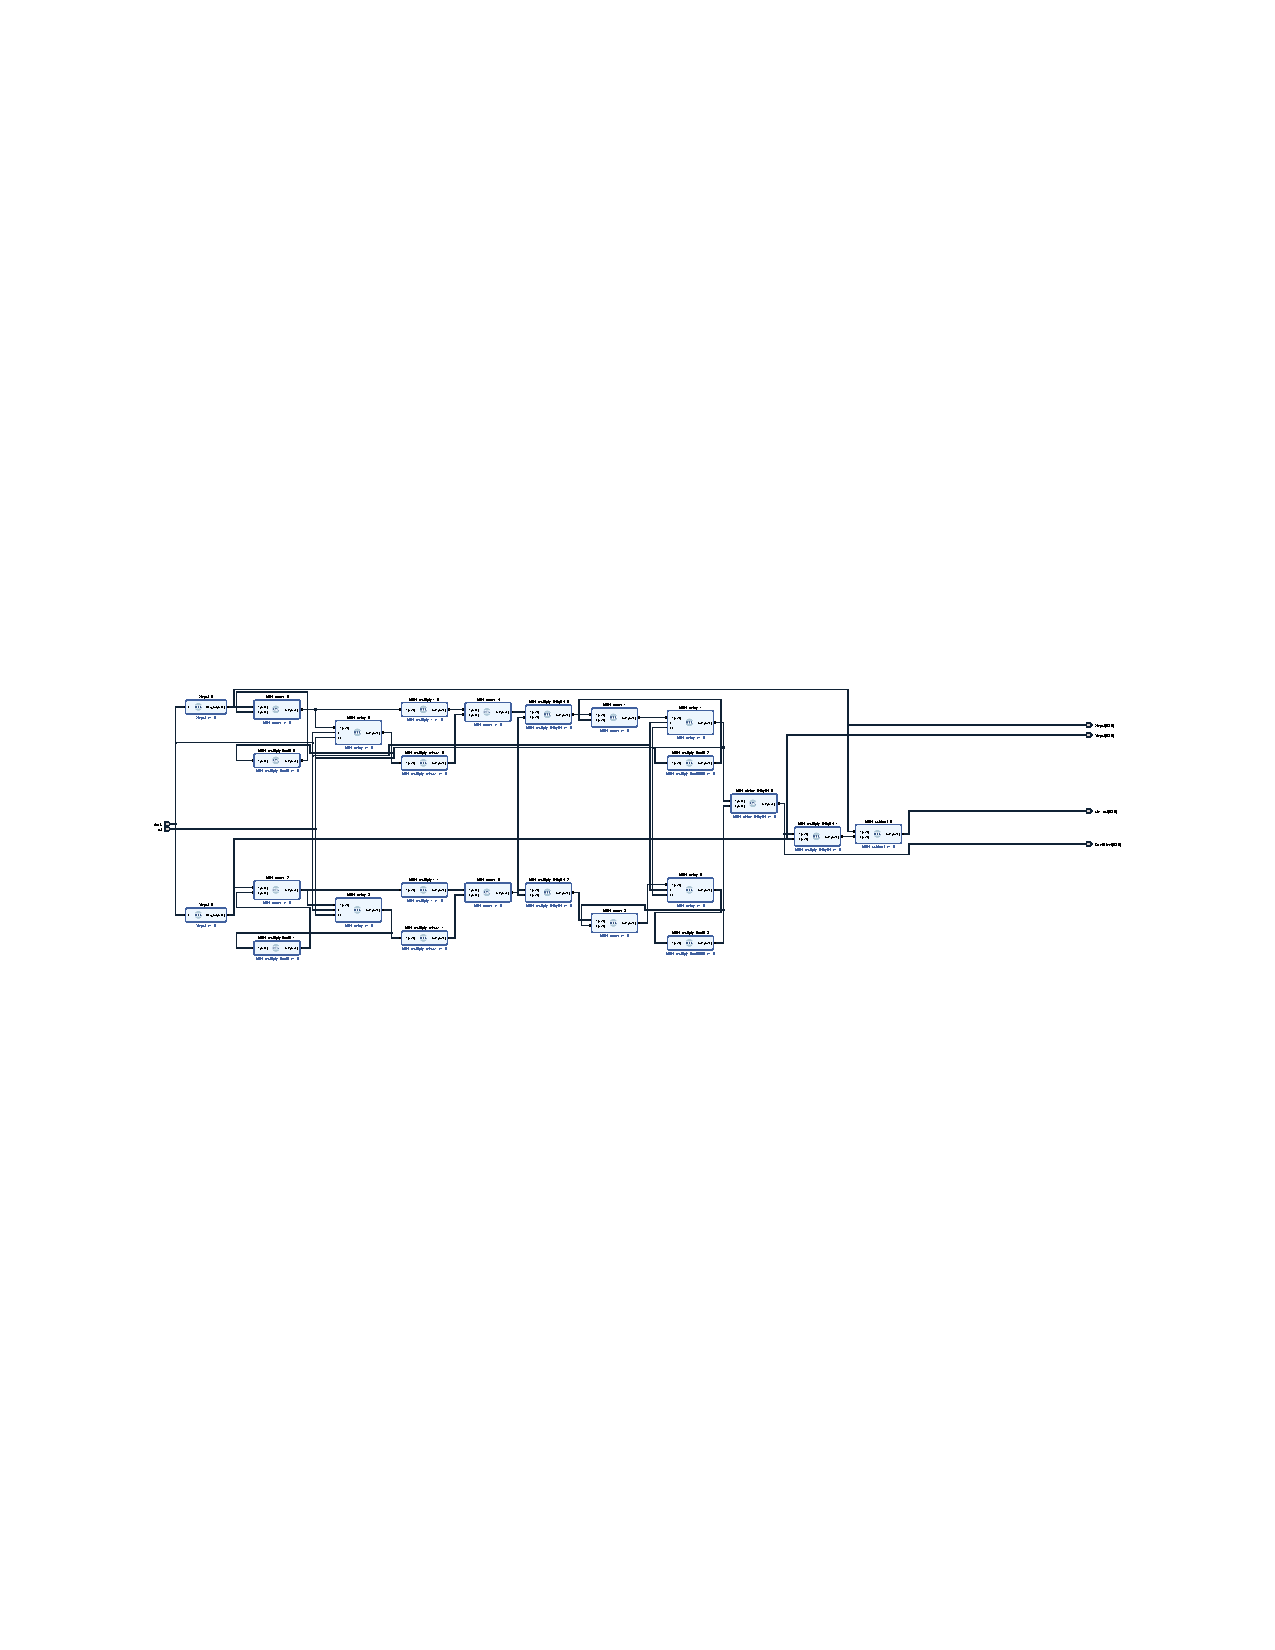
\includegraphics[width=1\linewidth]{4-ANC_Sys/VivadoBD_DSP.pdf}
\caption{Vivado DSP block diagram}
\label{fig_VivadoBD_DSP}
\end{figure}
\vfill
\end{landscape}

\begin{figure}[h]
\centering
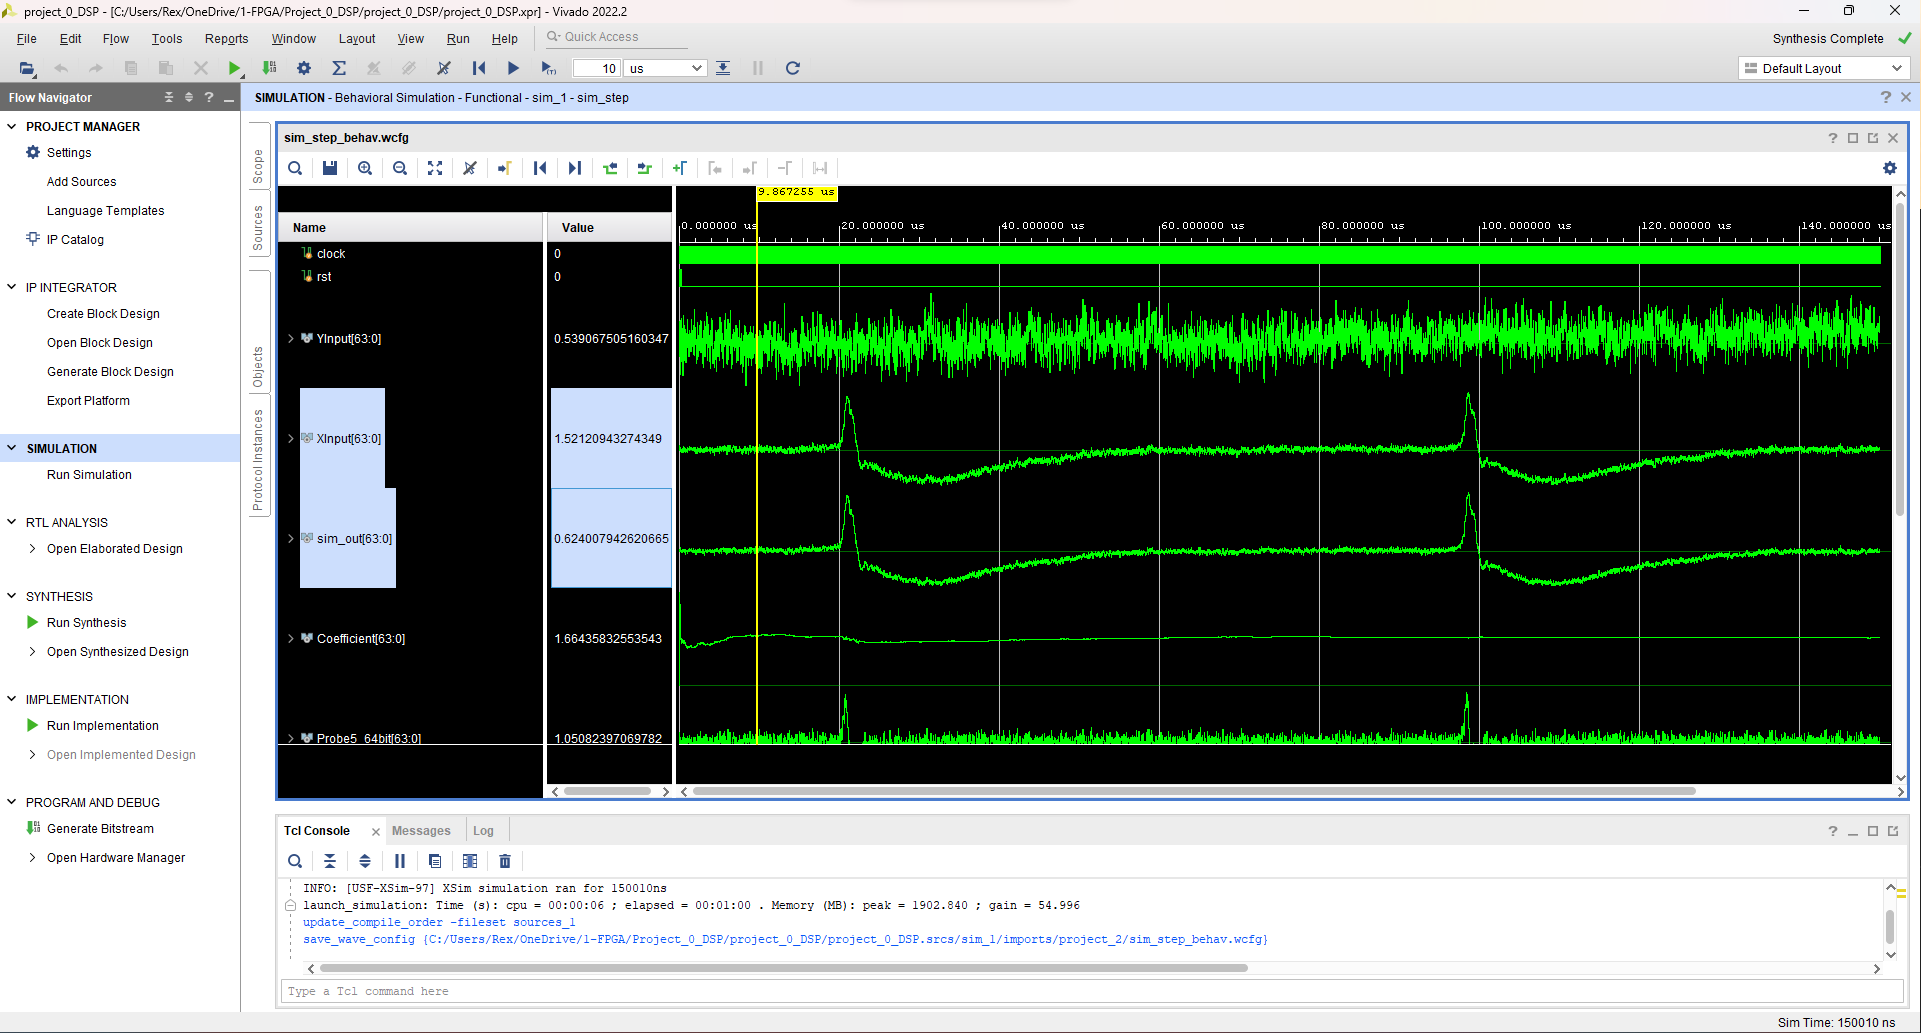
\includegraphics[width=1\linewidth]{4-ANC_Sys/VivadoSim.png}
\caption{Vivado simulation Result}
\label{fig_VivadoSimResult}
\end{figure}



\subsection{DSP block}



Applications such as brain-computer interfaces (BCIs), require arrays of hundreds of optrodes working together, with all processing done in real-time with FPGAs providing the best approach for such requirements.

We used a Wiener filter~\cite{WienerFilter} for preliminary investigations on pre-recorded optrode data to verify the effectiveness of actively cancelling in a realistic setup. However, in general Wiener filters process part of the signal one bin at a time and require a large amount of computational resources when the bin size gets large.  From experimental data, the optrode system showed little correlation between data streams beyond 3 samples from zero lag. We also determined that a one-tap filter showed significant noise reduction while increasing the number of taps showed little improvement.  This is fortunate, as an algorithm that must process hundreds of channels in real time, need to be simple and consume little power.  Therefore, a one-tap adaptive filter algorithm that is based on Wiener filtering has been designed and implemented on the FPGA board.

\begin{figure}[h]
\centerline{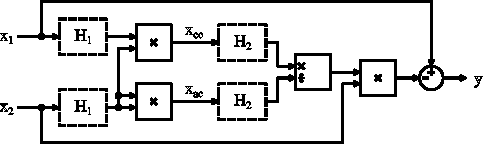
\includegraphics[width=1\linewidth]{4-ANC_Sys/DSP.pdf}}
\caption{Active noise cancelling algorithm block diagram.  It is an adaptive filter modified from the Wiener filter.}
\label{fig_DSP}
\end{figure}

Fig.~\ref{fig_DSP} shows the implemented digital signal processing infrastructure.  We assume here that the transfer function $H_1$ is common to both signals and that the transfer functions $H_2$ are identical integrators.  The system as shown has two inputs $x_1(i)$ and $x_2(i)$ respectively and a single output $y(i)$.  $x_1(i)$ carries the noisy message signal while $x_2(i)$ carries the noise signal.  The system is trying to remove the part of the noise in $x_1(i)$ that is correlated to the noise in $x_2(i)$, so we can posit:
$$x_1(i)=s(i)+n(i) \quad;\quad x_2(i)=m(i)+kn(i)$$
Where $n(i)$ is the part of the noise assumed present and correlated in both $x_1(i)$ and $x_2(i)$, $s(i)$ is signal plus random noise in $x_1(i)$, $m(i)$ is random noise in $x_2(i)$, and $k$ is the scale factor.  All of $s(i)$, $n(i)$, and $m(i)$ are random signals and assumed to be uncorrelated to each other.

Let $N$ be the total number of samples in $x_1(i)$ and $x_2(i)$.  Take $x_{cc}$, the cross-correlation of $x_1(i)$ and $x_2(i)$; and $x_{ac}$, the auto-correlation of $x_2(i)$, such that

$$x_{cc}(i)=\displaystyle\sum_{i=1}^{N} x_1(i)x_2(i), x_{ac}(i)=\displaystyle\sum_{i=1}^{N} x_2(i)x_2(i)$$
We divide the cross-correlation by the auto-correlation to get the filter coefficient:
\begin{equation}
\label{filterCoeff}
    \frac{x_{cc}(i)}{x_{ac}(i)} =\frac{\displaystyle\sum_{i=1}^{N} \left(s(i)m(i)+ks(i)n(i)+n(i)m(i)+n^2(i)k\right)}{\displaystyle\sum_{i=1}^{N} \left(m^2(i)+k^2n^2(i)+2km(i)n(i)\right)}
\end{equation}
Now, since $s(i)$, $n(i)$, and $m(i)$ are uncorrelated, all their respective cross-correlations should be equal to zero. In addition experiment results show that $kn(i)$ is the dominant noise in $x_2$, which means: 
$$
\sum_{i=1}^{N} k^2n^2(i) \gg \sum_{i=1}^{N} m^2(i)
$$
and consequently Eqn.~\ref{filterCoeff} reduces to:
$$
\frac{x_{cc}(i)}{x_{ac}(i)}=\frac{\displaystyle\sum_{i=1}^{N} kn^2(i)}{\displaystyle\sum_{i=1}^{N} m^2(i) + \displaystyle\sum_{i=1}^{N} k^2n^2(i)} \approx \frac{1}{k} 
$$
From this we can obtain the output $y(i)$:
\begin{align*}
    y(i)&=x_1(i)-\frac{1}{k}x_2(i) \\
    &=s(i)+n(i)-\frac{1}{k}m(i)-n(i)=s(i)-\frac{1}{k}m(i)
\end{align*}
Since $kn \gg m$, the noise level in $y$ is largely improved compared to $x_1(i)$.

To make the system more practical, a high-pass filter $H_1$ is implemented to remove any DC offset in the signals to improve cross-correlation and auto-correlation results.  A leaky integrator $H_2$ is used so the system has a moving average to track the most recent signal (in our case for about \qty{500}{ms}).  This leaky integrator compensates for the potential changes in the gain of $x_1(i)$ and $x_2(i)$ caused by {\em e.g.} temperature change or physical movement.

\begin{figure*}[h]
\centerline{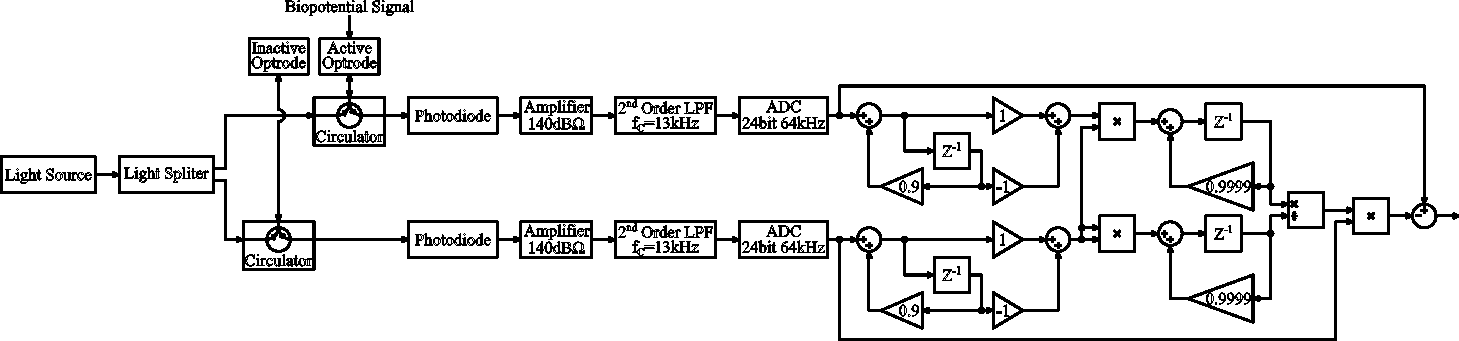
\includegraphics[width=1\linewidth]{4-ANC_Sys/DataFlow.pdf}}
\caption{Data flow block diagram.  Light from a light source is split into two channels of light, one goes to the active optrode and measures nerve signal, and the other one goes to the inactive optrode and does not measure anything.  The two channels of light are then converted to digital signals and are processed by a DSP algorithm.}
\label{fig_DataFlow}
\end{figure*}

Fig.~\ref{fig_DataFlow} shows the data flows as currently implemented.  Light comes out of a light source and is split into two identical signals at the passive light splitter.  Then one signal goes to the active optrode where it measures a nerve signal, and the other signal goes to an inactive optrode and carries no extra information.  Both signals are converted into current by the photodiode, then converted into voltage by the amplifier, and finally converted into digital signals by the ADC, which all happen on the light receiver board.  Finally, the digital signals are transmitted to the FPGA for digital signal processing.

In our case, the light source is a super-luminescent diode with a \qty{1550}{\nm} wavelength, and a variable current of up to \qty{800}{\mA}, running at a constant temperature of \qty{20}{\degreeCelsius}.  The frequency range of the nerve signal is \qty{10}{\Hz} to \qty{10}{\kHz}.  The light receiver board gain is set to \qty{140}{dB\Omega} for all the measurements.  The USB serial port embedded in the FPGA board can only stream the data to a PC at 300Hz, which does not meet the requirement.  However, it is capable to stream out real-time data at \qty{64}{kHz} with suitable peripherals.  In this project, an SD card is used to store data to save development time.

\subsection{FPGA}

The FPGA board used in this project is shown in fig.~\ref{fig_FPGA}.  There is a Xininx Zynq 7020 SoC on board.  The Xilinx Zynq 7020 is part of the Zynq-7000 family, which represents a class of products known as All Programmable System-on-Chips (APSoCs). These devices combine the software programmability of an ARM Cortex-A9 dual-core processor with the hardware programmability of an FPGA, providing a unique platform that suits our needs.  While the FPGA can handle all the functions we need, an onboard microcontroller is a lot easier to use for functions like controlling the gain.  The board also has high-speed IO pins as we need them to read from the ADC at the speed of \qty{24}{bit} and \qty{64}{kHz}, which requires at least \qty{1.536}{MHz} clock speed for the SPI port.  There are also buttons and LEDs for input and status indication.  There is also a serial port going through the USB port that could be used for data streaming to a PC.  However, upon testing it shows only capable of streaming 2 channels \qty{24}{bit} data at \qty{400}{Hz}.  Therefore, we decided to use an SD card to store data.

\begin{figure}[h]
\centering
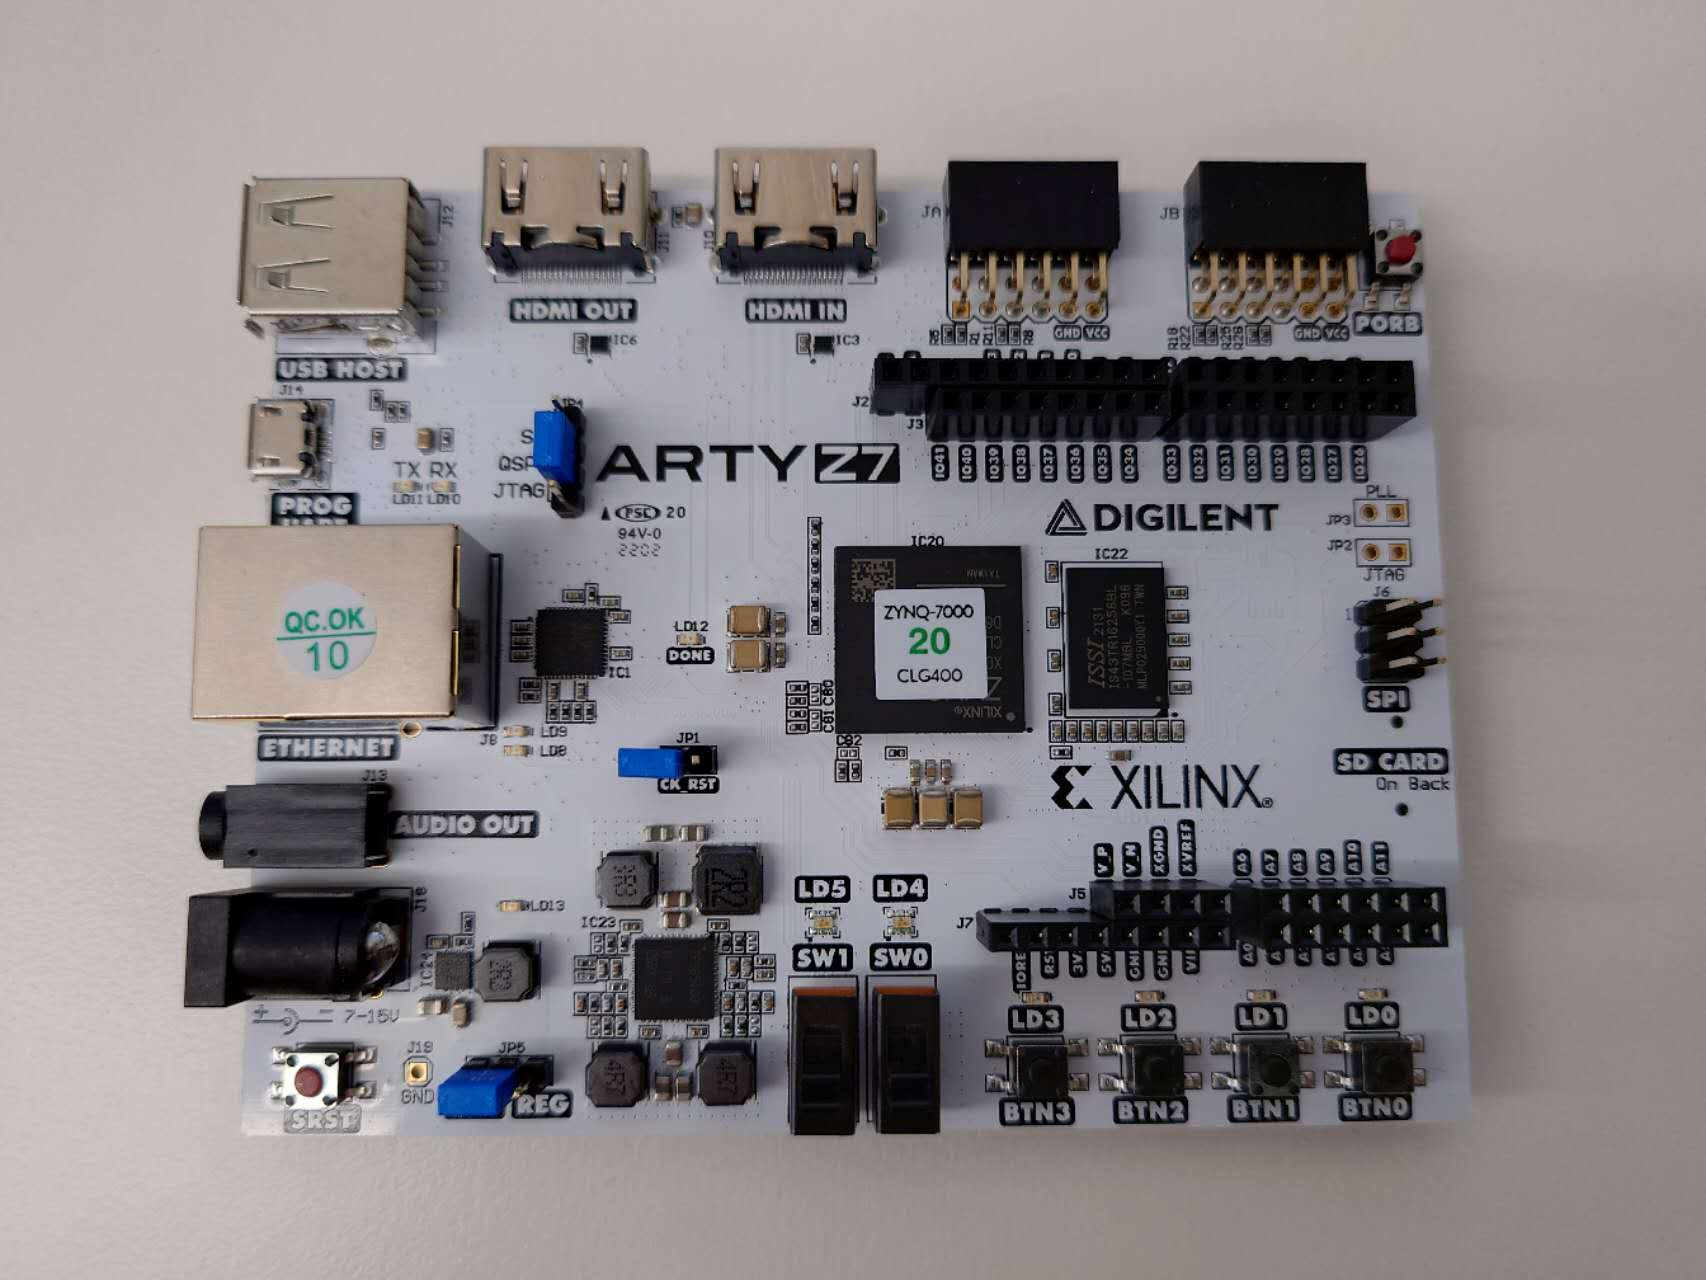
\includegraphics[width=1\linewidth]{4-ANC_Sys/FPGA.jpg}
\caption{FPGA}
\label{fig_FPGA}
\end{figure}

Fig.~\ref{fig_VivadoBD_DSP_onFPGA} shows the noise cancelling DSP algorithm in the Vivado block diagram, that is been implemented in the FPGA.  The difference between this diagram to the simulation diagram shown in fig.~\ref{fig_VivadoBD_DSP}, is the input data.  The ADC on the light receiver board outputs \qty{24}{bit} unsigned integer that represents a voltage level between $V_{ref-}$ and $V_{ref+}$, which is slightly different to the form of \qty{16}{bit} biomedical data used before.  The decimal point is still placed in the middle of the \qty{64}{bit} number.  To avoid overflow when performing multiply calculations, we are placing the \qty{24}{bit} number right after the decimal point.  For example, a \qty{24}{bit} number $\mathtt{0x123abc}$ will be placed at $\mathtt{0x00000000.123abc00}$.  When mapping the \qty{24}{bit} number into the \qty{64}{bit} number, the signed and virtual ground is also added.  On the light receiver board, the reference voltage for all the amplifier and filter circuits is \qty{2.1}{V}, which serves as a virtual ground.  When processing in the algorithm, the data has to be centred around zero, so we have to subtract the virtual ground before the data enters the algorithm.  Also, the algorithm calculation is signed, and the ADC data input is unsigned.  To change both the sign and virtual ground at the same time, we can simply use the mapped number to subtract a signed virtual ground number $\mathtt{00000000AACCCCCD}$.  The output is been mapped back from \qty{64}{bit} to \qty{24}{bit} as well.

\begin{landscape}\centering
\vspace*{\fill}
\begin{figure}[h]
\centerline{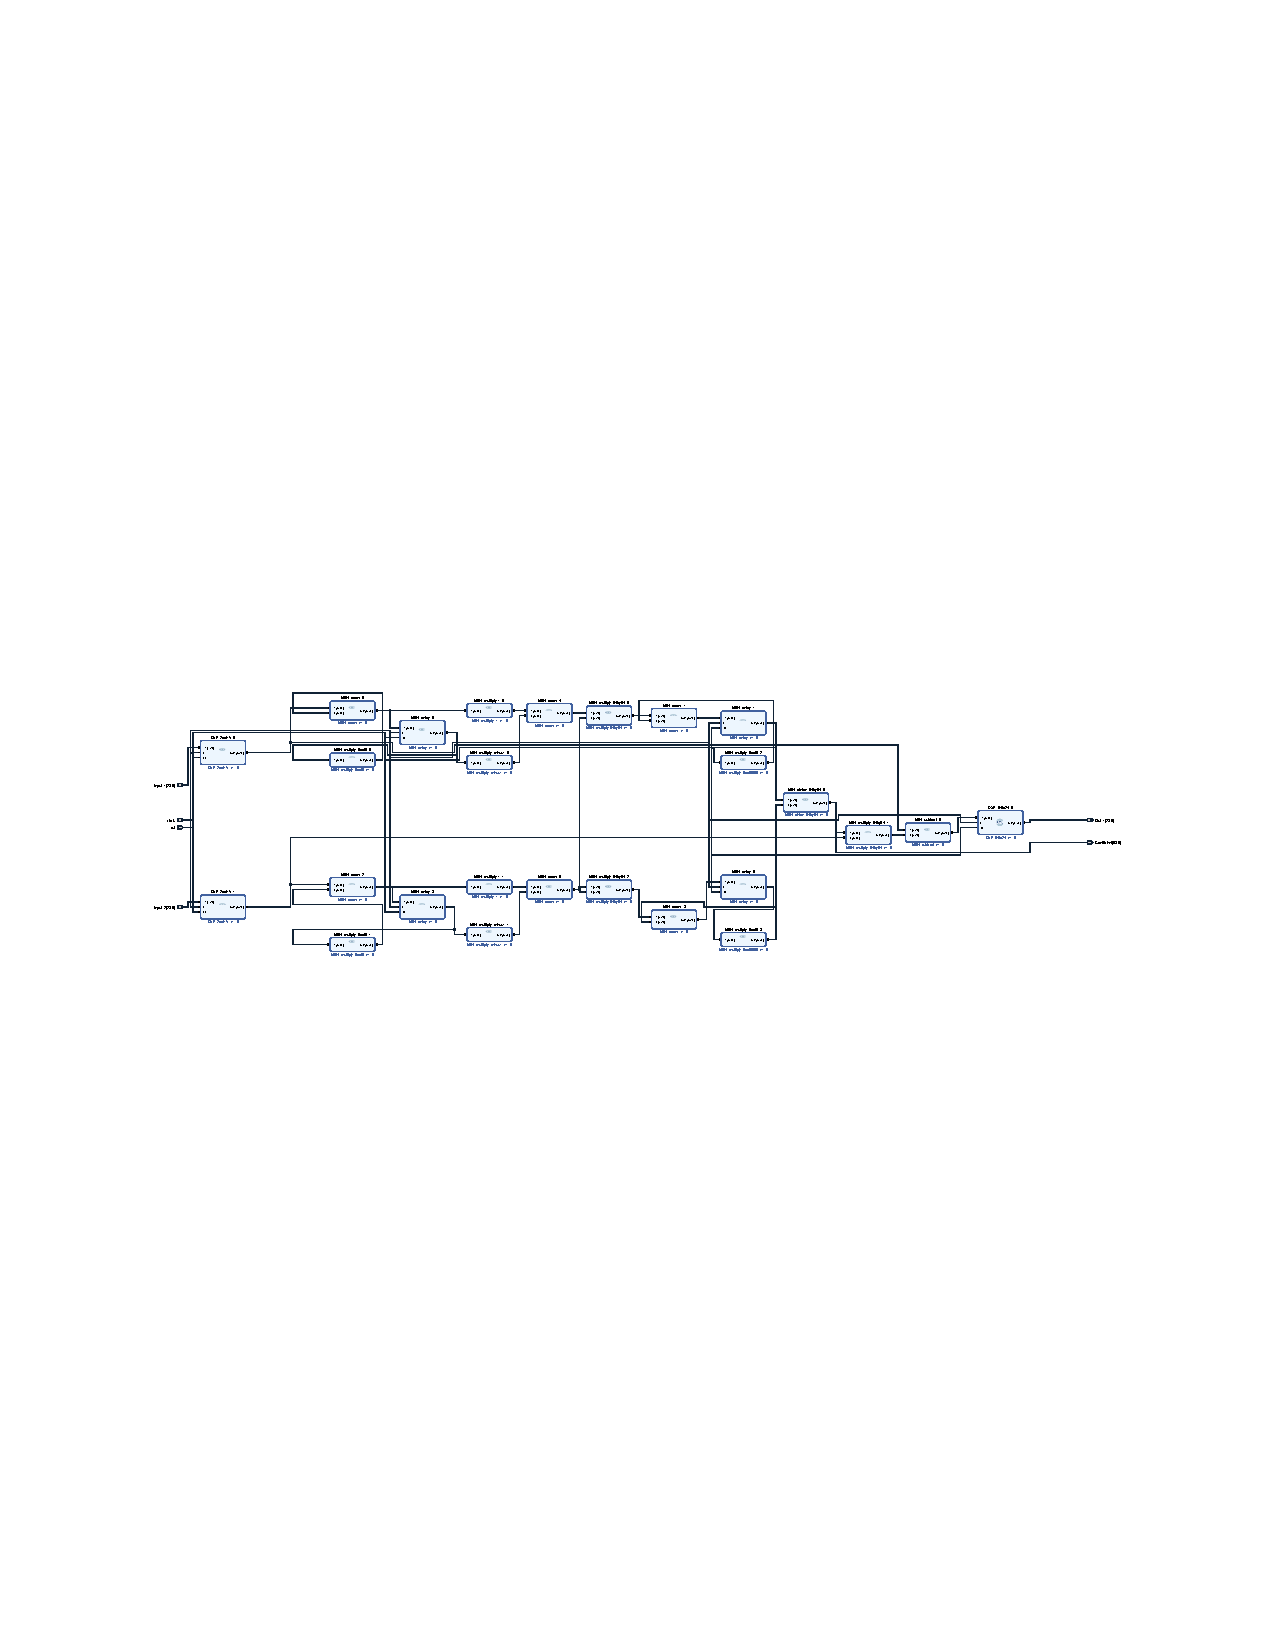
\includegraphics[width=1\linewidth]{4-ANC_Sys/VivadoBD_DSP_onFPGA.pdf}}
\caption{Vivado DSP Block Diagram}
\label{fig_VivadoBD_DSP_onFPGA}
\end{figure}
\vfill
\end{landscape}

\begin{figure}[h]
\centerline{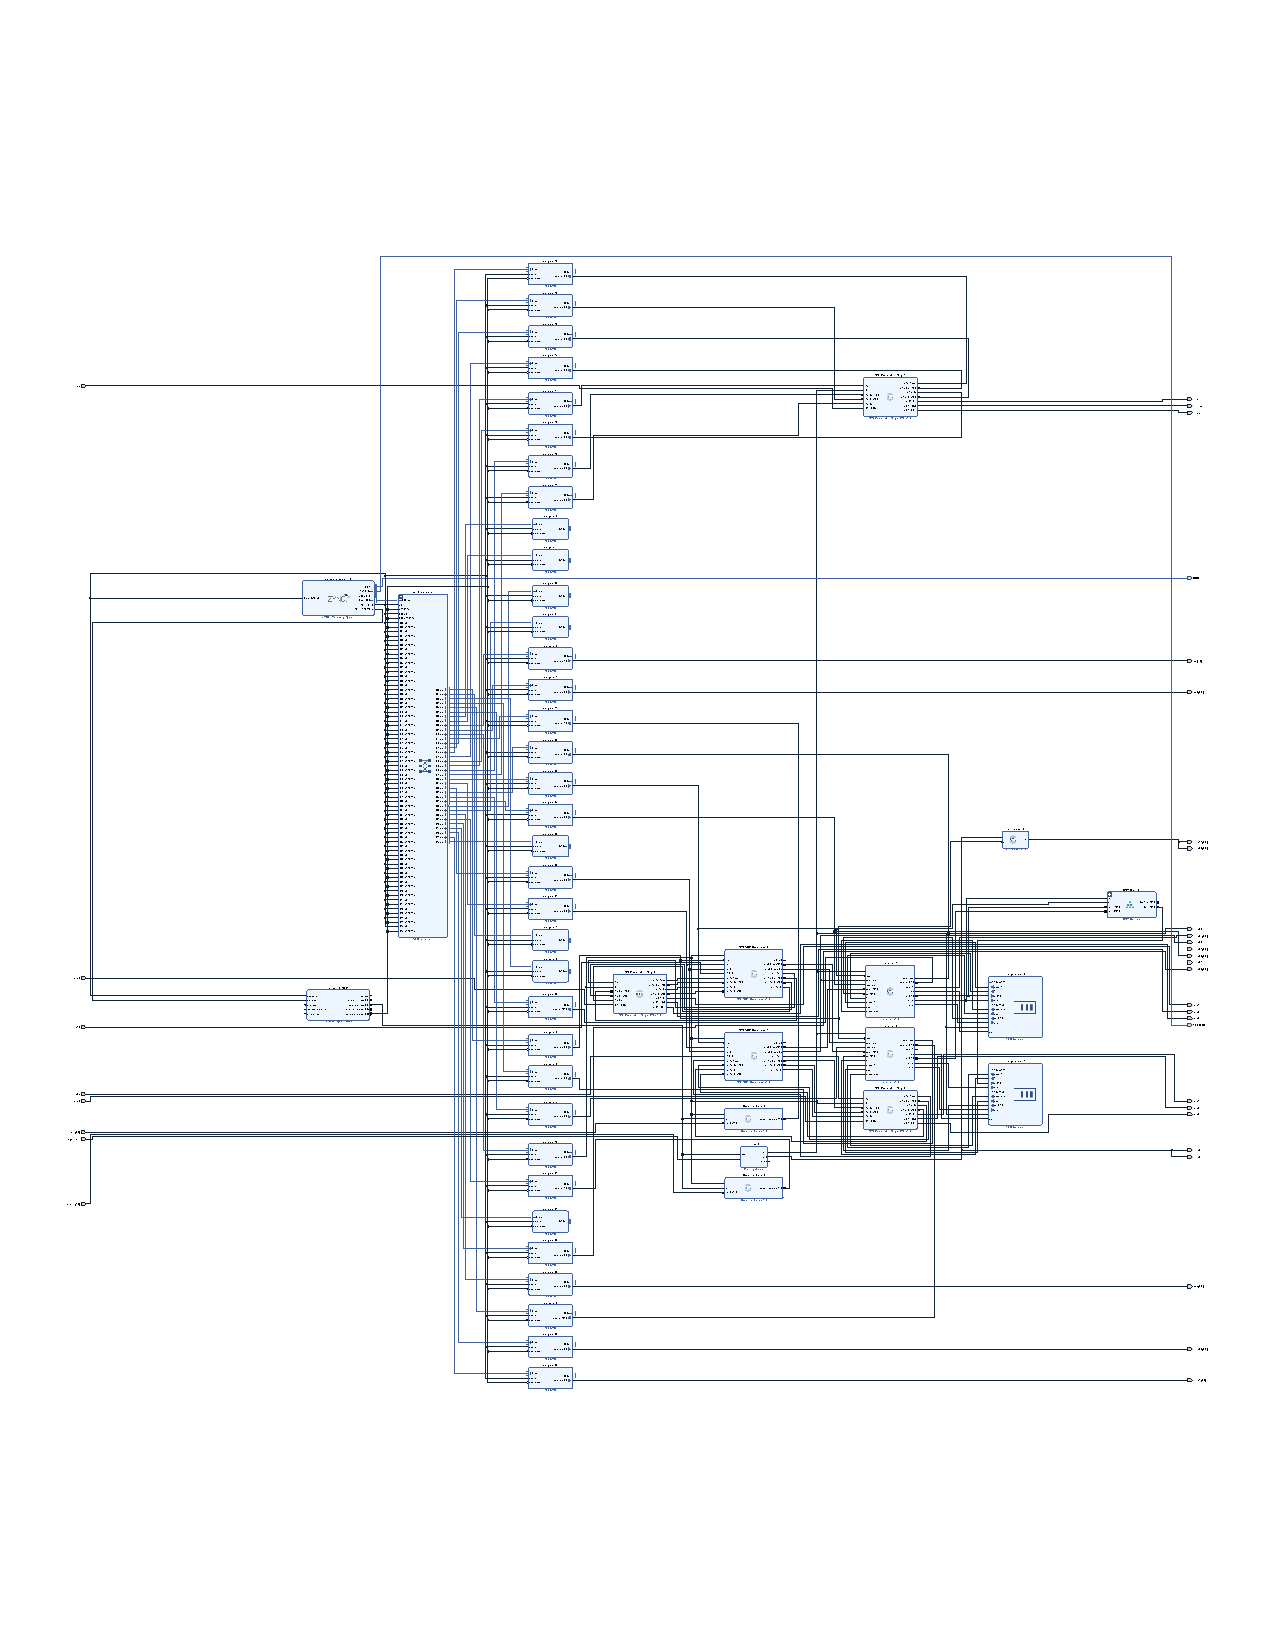
\includegraphics[width=1\linewidth]{4-ANC_Sys/VivadoBD.pdf}}
\caption{Vivado Block Diagram}
\label{fig_VivadoBD}
\end{figure}

\begin{landscape}\centering
\begin{figure}[h]
\centerline{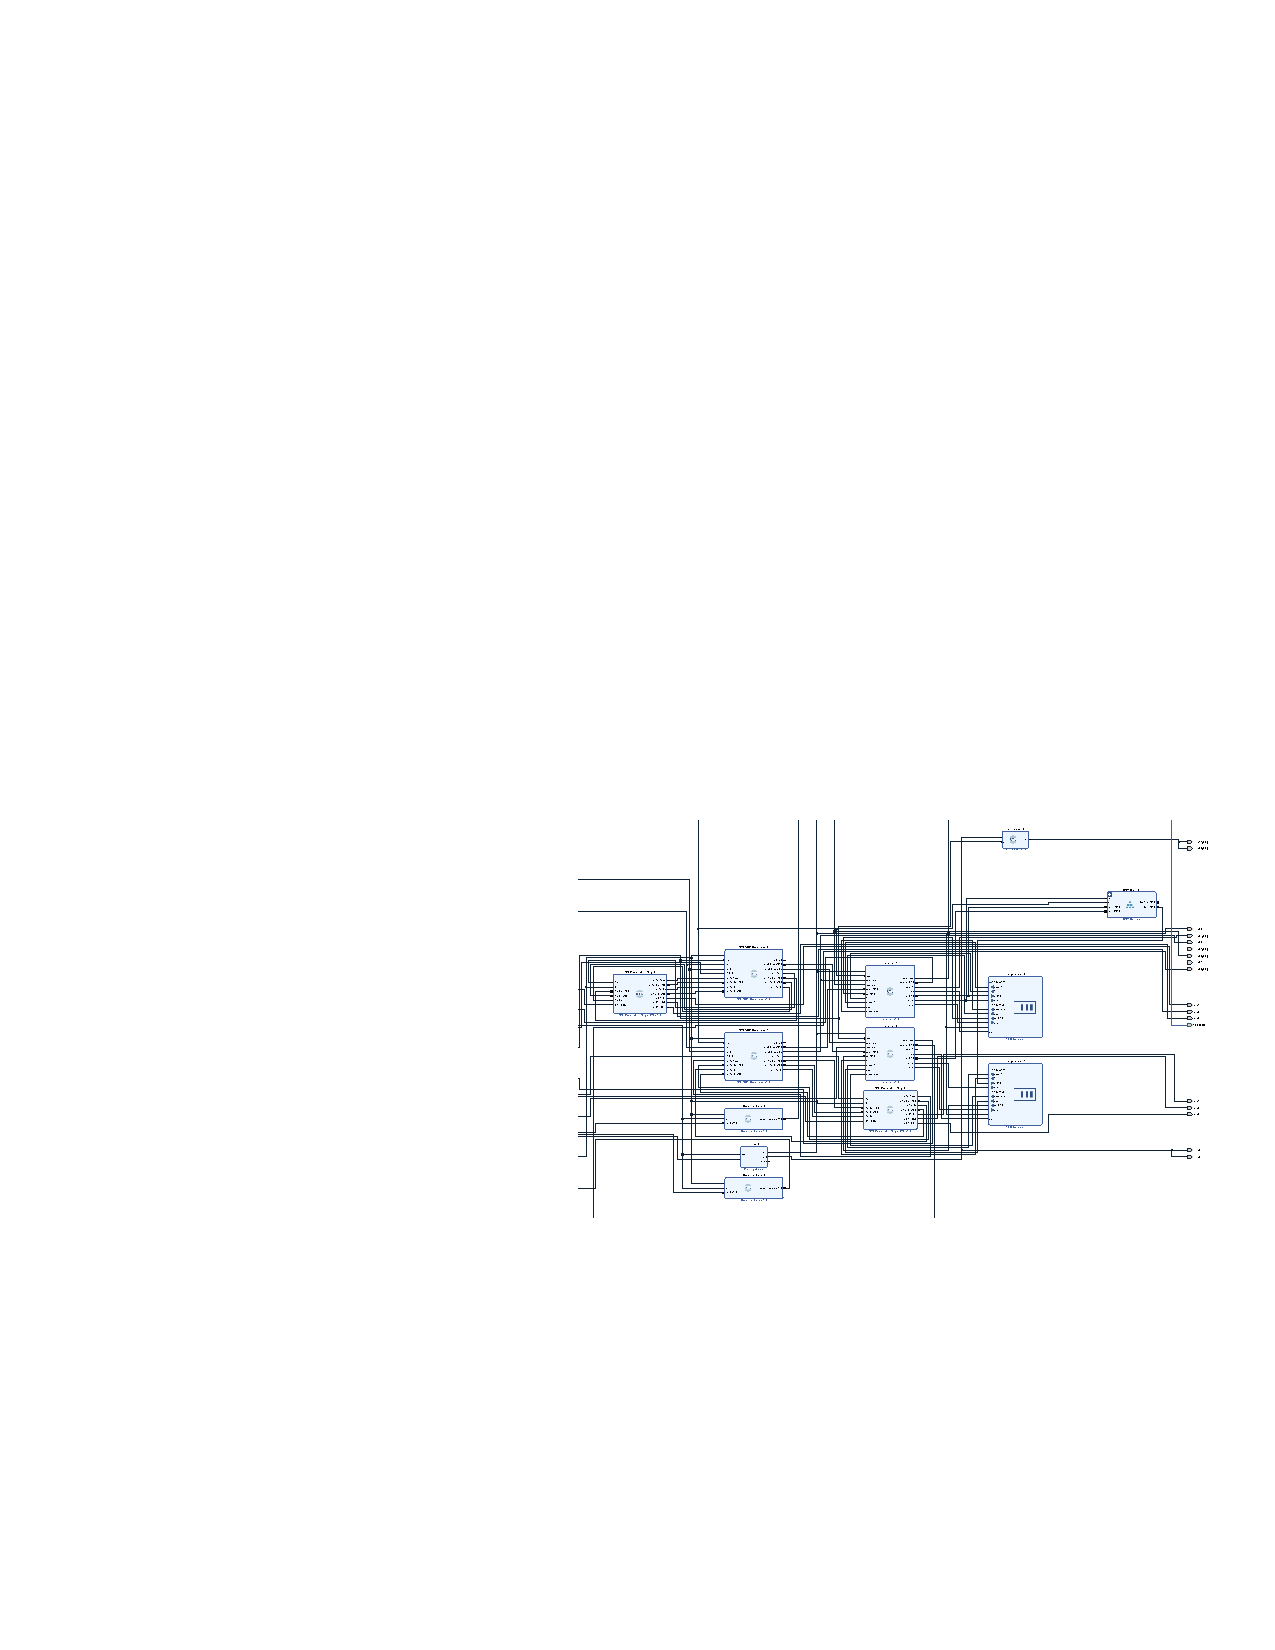
\includegraphics[scale=2]{4-ANC_Sys/VivadoBD_ZoomIn.pdf}}
\caption{Vivado Block Diagram Zoom In}
\label{fig_VivadoBD_ZoomIn}
\end{figure}
\end{landscape}

The whole block diagram for the FPGA structure is shown in fig.~\ref{fig_VivadoBD}.  Since it is very complicated, a zoom-in to the bottom right is shown in fig.~\ref{fig_VivadoBD_ZoomIn}.  On the left half of fig.~\ref{fig_VivadoBD} is the connection block between the FPGA and the microcontroller.  The C code in the microcontroller is shown in the Appendix~\ref{a:codes}.  When the system powers on, the microcontroller starts to execute the C code.  In the C code, there is firstly a setting while loop to ask for gain setting, which can be set using the button and switch on the FPGA board.  The new gain setting will be transferred to the $SPI\_Master\_With\_Sing\_1$ block on the top right corner of fig.~\ref{fig_VivadoBD} and then transmitted to the digital potentiometer to update the resistance setting in it therefore changing the gain.  There are three $SPI\_Master$ blocks in the block diagram, the code for these blocks is downloaded from the internet.  They receive commands from another block to send out data string with SPI standard and send the returning data back to another block.  After setting the gain to a proper value, flipping on a switch triggers another reading while loop to start reading and storing the ADC and DSP data.  The reading while loop sends a signal to start $SPI\_ADC\_Read\_Loop\_0$ and $SPI\_ADC\_Read\_Loop\_1$, which then control the other two $SPI\_Master$ blocks to read the ADC whenever a sample is ready.  The $SPI\_Master$ blocks send the returning ADC data into the DSP algorithm block and perform active noise cancelling.  Then the active optrode data channel and the DSP algorithm output channel are put through to a FIFO buffer.  The reading while loop reads the FIFO buffer when the buffer is not empty and writes the data into the SD card.  The reason to use a buffer is that the SD card can only be read or written by the microcontroller, and not the FPGA.  While the microcontroller is running at a fast frequency, it is sticking in somewhere for a while from time to time.  This means that the microcontroller will miss data if we just use the loop to scan.  Therefore, a FIFO buffer is needed to give the microcontroller buffer time to execute other things.  As long as the average reading and writing speed of the microcontroller is faster than the sampling rate, all the data can be safely written into the SD card.

The utilization report of the FPGA is shown in tab~\ref{tab_FPGAUtilSimple}, and a more detailed version can be found in the appendix~\ref{a:FPGA}.  This report shows that 63\% LUT in the FPGA are used, which is 33571 LUTs out of 53200 LUTs in total.  The DSP algorithm alone takes 30024 LUTs, which is a lot.  There are four of multiply by 0.9 blocks each taking about 5000 LUTs, and one divide block taking 9000 LUTs.  These five blocks combined already take up half the FPGA LUTs, so if we want more filter taps, the algorithm will need to be optimized to compress the size.

% Please add the following required packages to your document preamble:
% \usepackage[table,xcdraw]{xcolor}
% If you use beamer only pass "xcolor=table" option, i.e. \documentclass[xcolor=table]{beamer}
% \usepackage{longtable}
% Note: It may be necessary to compile the document several times to get a multi-page table to line up properly
\begin{longtable}[c]{|l|l|l|l|}
\hline
\textbf{Resource} & \textbf{Utilization} & \textbf{Available} & \textbf{Utilization \%} \\ \hline
\endhead
%
\rowcolor[HTML]{FFFFFF} 
LUT & 33571 & 53200 & 63.10 \\ \hline
\rowcolor[HTML]{FFFFFF} 
LUTRAM & 62 & 17400 & 0.36 \\ \hline
\rowcolor[HTML]{FFFFFF} 
FF & 4253 & 106400 & 4.00 \\ \hline
\rowcolor[HTML]{FFFFFF} 
BRAM & 22 & 140 & 15.71 \\ \hline
\rowcolor[HTML]{FFFFFF} 
DSP & 40 & 220 & 18.18 \\ \hline
\rowcolor[HTML]{FFFFFF} 
IO & 44 & 125 & 35.20 \\ \hline
\rowcolor[HTML]{FFFFFF} 
MMCM & 1 & 4 & 25.00 \\ \hline
\caption{Utilization of FPGA}
\label{tab_FPGAUtilSimple}\\
\end{longtable}

\section{Complete system}

Fig.~\ref{fig_BoardCon} shows the connection between the two boards.  Cables with dedicated connectors are made for easier connecting and better signal integrity.  The two parallel cable goes from top and bottom of receiver board to the two Pmod port on the FPGA board runs the high speed SPI signal, and the cable that runs to the arduino-alike port on the FPGA board is running the lower speed SPI control signal.  The white cable runs the SPI that controls the digital potentiometer.



\begin{figure}[h]
\centering
\begin{subfigure}{.5\textwidth}
  \centering
  \includegraphics[width=0.9\linewidth]{4-ANC_Sys/BoardCon_1.jpg}
  \caption{}
  \label{fig_BoardCon_1}
\end{subfigure}%
\begin{subfigure}{.5\textwidth}
  \centering
  \includegraphics[width=0.9\linewidth]{4-ANC_Sys/BoardCon_2.jpg}
  \caption{}
  \label{fig_BoardCon_2}
\end{subfigure}
\caption{Light receiver board and FPGA board connection}
\label{fig_BoardCon}
\end{figure}

To use the complete active noise cancelling system for Optrode, firstly connect \qty{12}{V} battery to the power pins of the light receiver board, then connect a USB cable from a laptop to power the FPGA board.  Make sure the laptop is powered by its own battery, and the boot inmage is loaded in the SD card.  Then, use $BTN0$ to increase and $BTN1$ to decrease the gain setting, $LD0$ to $LD4$ will display the current gain setting, tab~\ref{tab_GainDisplay} shows how the LEDs displays the gain.  After completeing the gain set up, use $SW0$ to update the settings to the light receiver board.  To start recording, switch on $SW1$, and The data received will be written into the SD card.  Switch off $SW0$ to stop the recording and download the data from SD card.  A more detailed manual and MATLAB codes used for reading the data is shown in Appendix~\ref{a:manual}.

\begin{table}[h]
\centering
\begin{tabular}{|l|l|l|l|l|}
\hline
\textbf{} & \multicolumn{1}{c|}{LD3} & \multicolumn{1}{c|}{LD2} & \multicolumn{1}{c|}{LD1} & \multicolumn{1}{c|}{LD0} \\ \hline
110dB & 0 & 0 & 0 & 1 \\ \hline
120dB & 0 & 0 & 1 & 1 \\ \hline
130dB & 0 & 1 & 1 & 1 \\ \hline
140dB & 1 & 1 & 1 & 1 \\ \hline
\end{tabular}
\caption{Gain Display}
\label{tab_GainDisplay}
\end{table}
